%=================================================================
\documentclass{ieeeaccess}

\usepackage{booktabs}
\usepackage{multirow}
\usepackage{array}
\usepackage{graphicx}
\usepackage{amssymb}
\usepackage{amsmath}
\usepackage{textcomp}
\usepackage{float}
\usepackage{url}
\usepackage[capitalize]{cleveref}
\graphicspath{{figures/}}

% Workaround: ieeeaccess.cls redefines \textbf via plain-TeX \bf, which
% breaks \textbf{$...$} in math mode; use \bfseries-based definition instead.
\renewcommand{\textbf}[1]{{\bfseries #1}}

\newcommand{\orcidauthorA}{0009-0002-5071-0054}
\newcommand{\orcidauthorB}{0009-0004-0749-3239}

\begin{document}
\history{Date of publication xxxx 00, 0000, date of current version xxxx 00, 0000.}
\doi{10.1109/ACCESS.2024.0429000}

\title{AnchorScore: A CLIP-Based Diagnostic of MLLM Annotation Difficulty in Classroom Behavior Analysis}

\author{\uppercase{Yan Ma}\authorrefmark{1}\authorrefmark{2},
\uppercase{Lizhuo Zhang}\authorrefmark{3}}

\address[1]{School of Foreign Studies, Changsha University of Science and Technology, Changsha 410114, China (e-mail: mayan@csust.edu.cn)}
\address[2]{School of Education, Hunan Agricultural University, Changsha 410128, China}
\address[3]{School of Information and Intelligence, Hunan Agricultural University, Changsha 410128, China (e-mail: zhanglizhuo@hunau.edu.cn)}
\tfootnote{This research received no external funding.}
\markboth
{Ma and Zhang: AnchorScore: A CLIP-Based Diagnostic of MLLM Annotation}
{Ma and Zhang: AnchorScore: A CLIP-Based Diagnostic of MLLM Annotation}
\corresp{Corresponding author: Lizhuo Zhang (e-mail: zhanglizhuo@hunau.edu.cn).}
\titlepgskip=-15pt

\begin{abstract}%
Multimodal large language models (MLLMs) are widely used for automated annotation, yet their per-class accuracy varies widely (12\%--98\%) and is expensive to measure: evaluating one MLLM takes roughly 14 hours, while CLIP inference completes in 3 minutes. No cheap a priori signal currently identifies where an MLLM will struggle. We introduce \textbf{AnchorScore}, the per-class zero-shot accuracy of a frozen CLIP model, as a lightweight diagnostic that flags the classes MLLMs are least likely to annotate reliably.

On classroom behavior data (SCB5, 13 classes, 6 MLLMs), AnchorScore correlates with per-class MLLM accuracy (Spearman $\rho=0.769$, $p=0.002$, $n=13$). None of the alternative difficulty predictors we evaluated (DINOv2, ResNet-50, SigLIP, or MLLM self-verbalized uncertainty) showed a significant correlation. A cross-model consensus control suggests AnchorScore captures a shared class-difficulty factor rather than a CLIP-specific signal: conditioning on the consensus of the other five MLLMs leaves a partial correlation statistically indistinguishable from zero. An independent replication on Stanford40 Actions yields a nearly identical effect ($\rho=0.817$, $p<0.001$).

Three practical applications follow: an AnchorScore-based hybrid CLIP/MLLM annotation strategy (up to $+$11~pp at roughly half the MLLM cost), prompt disambiguation on hard classes, and review-priority prediction for human verification. AnchorScore does not estimate exact MLLM accuracy; it provides a low-cost ranking signal that directs expensive MLLM evaluation to the classes where it is most informative.
\end{abstract}

\begin{keywords}
CLIP; multimodal large language models; zero-shot evaluation; active learning; annotation reliability
\end{keywords}

\maketitle

\section{Introduction}
\label{sec:intro}

Multimodal large language models (MLLMs) are now widely adopted for automatic data annotation~\cite{liu2023visual}. Their per-class accuracy, however, varies dramatically. On a classroom behavior dataset (SCB5)~\cite{ma2026agreement}, annotation accuracy averaged across six MLLMs exceeds 97\% for ``blackboard-writing'' but reaches only 12\% for ``answer'', a gap of 85~pp (percentage points). Without running the full annotation pipeline on tens of billions of parameters, how can practitioners identify which classes an MLLM will annotate reliably?

Existing approaches, such as running a pilot sample through the MLLM or extracting model-specific uncertainty~\cite{kadavath2022language}, remain computationally expensive. Evaluating one 27B MLLM on 5,416 validation images takes roughly 14 hours, while requiring access to the model itself. We propose a lightweight alternative: \textbf{AnchorScore}, defined as the per-class zero-shot accuracy of a frozen CLIP model~\cite{radford2021clip}. If CLIP's zero-shot accuracy on a class is low, will a larger MLLM (26--35B parameters) also struggle? A single CLIP forward pass in 3 minutes can reveal which classes are likely to challenge the MLLM, producing a per-class difficulty map that would otherwise require hours of MLLM inference.

Validation on SCB5 (13 classes, 6 MLLMs) shows a significant class-level correlation between AnchorScore and MLLM accuracy ($\rho=0.769$, $p=0.002$). Alternative probes (SigLIP, DINOv2, ResNet-50, MLLM self-uncertainty) show no significant correlation, and a consensus control indicates the signal reflects a shared class-difficulty factor rather than a CLIP-specific mechanism. An independent replication on Stanford40 Actions (40 classes, $\rho=0.817$) confirms the effect. Three practical applications follow from this diagnostic: hybrid CLIP/MLLM annotation routing, prompt disambiguation guided by CLIP confusion patterns, and review-priority ranking.

AnchorScore is not a calibrated accuracy estimator; it is a low-cost diagnostic for ranking classes by relative difficulty. The contributions are threefold:
\begin{itemize}
\item \textbf{Diagnostic discovery.} We show that a cheap, training-free probe from a \emph{different} model family---frozen-CLIP per-class zero-shot accuracy---predicts where MLLM annotation is unreliable, correlating with per-class MLLM accuracy on SCB5 ($\rho=0.769$, $p=0.002$) and replicating on Stanford40 ($\rho=0.817$, $p<0.001$). This is not a claim that ``CLIP knows difficulty''; the value is that the signal is obtainable before any MLLM inference, turning MLLM evaluation from a per-model cost into an allocatable budget.
\item \textbf{Mechanism clarification.} Alternative difficulty predictors (SigLIP, DINOv2, ResNet-50, MLLM self-uncertainty) show no significant correlation, and a cross-model consensus control indicates the signal reflects a \emph{shared} class-difficulty factor rather than a CLIP-specific mechanism.
\item \textbf{Practical uses.} The signal supports a \emph{screening-routing-disambiguation-review} pipeline: hybrid CLIP/MLLM annotation, confusion-guided prompt disambiguation, and review-priority prediction.
\end{itemize}
Our contribution is empirical rather than algorithmic: AnchorScore is simply CLIP zero-shot accuracy, and its value lies in the evidence chain establishing when and where this diagnostic is reliable.

\section{Method}
\label{sec:method}

The AnchorScore pipeline proceeds as follows.

\subsection{AnchorScore Definition}

AnchorScore measures the per-class zero-shot accuracy of a CLIP model on a target dataset. For a dataset with $C$ classes $\{c_1, c_2, \dots, c_C\}$ and a validation set of $N$ images, we compute:

\begin{equation}
\text{AnchorScore}(c_i) = \frac{1}{N_i} \sum_{j : y_j = i} \mathbb{1}[\hat{y}_j = y_j]
\label{eq:anchorscore}
\end{equation}

where $j$ indexes the $N$ validation images, $N_i$ is the number of validation images of class $c_i$ (the label $y_j$ equals $i$ for exactly $N_i$ of the $N$ images), $y_j$ and $\hat{y}_j$ are the ground-truth label and the CLIP prediction for image $j$, both encoded as class indices in $\{1,\dots,C\}$, and $\mathbb{1}[\cdot]$ is the indicator function: it equals 1 when the CLIP prediction matches the ground-truth label and 0 otherwise. The sum therefore counts the images of class $c_i$ that CLIP classifies correctly, and $\text{AnchorScore}(c_i)$ is the fraction of such images---CLIP's per-class zero-shot accuracy. It serves as a low-cost proxy of the class-level difficulty and is the difficulty signal used throughout the correlation analyses in \Cref{sec:experiments}. The CLIP prediction is defined as:

\begin{equation}
\hat{y}_j = \arg\max_{k \in \{1,\dots,C\}} \frac{\mathbf{f}_{\text{img}}(x_j)^\top \bar{\mathbf{f}}_{\text{text}}(c_k)}{\|\mathbf{f}_{\text{img}}(x_j)\| \|\bar{\mathbf{f}}_{\text{text}}(c_k)\|}
\label{eq:clip_pred}
\end{equation}

Here $\mathbf{f}_{\text{img}}$ and $\mathbf{f}_{\text{text}}$ are the CLIP vision and text encoders, $x_j$ is the input image, and $p_k$ is the text prompt for class $c_k$. Following template averaging, $\bar{\mathbf{f}}_{\text{text}}(c_k) = \frac{1}{T}\sum_{t=1}^{T}\mathbf{f}_{\text{text}}(p_{k,t})$ denotes the mean text embedding of class $c_k$ across $T$ prompt templates $p_{k,1}, \dots, p_{k,T}$, with $T=3$ in our experiments.

\subsection{Prompt Design}

To improve robustness without adding computational overhead, we average text features over $T=3$ prompt templates for classroom datasets, following the template-averaging strategy of the Smart Classroom Behavior (SCB5) benchmark~\cite{scb_dataset}. We verified that using only the first prompt ($T=1$) yields a consistently lower but still positive correlation at the class level, confirming that multi-prompt averaging adds marginal but consistent benefit:

{\footnotesize
\begin{verbatim}
[ "a photo of a person {cls} in classroom.",
  "a classroom scene showing {cls}.",
  "the action of {cls} in a school environment." ]
\end{verbatim}}

For cross-domain datasets, we use domain-specific prompts (e.g., ``a satellite image of {cls}'' for EuroSAT). For classes with ambiguous names, we apply a manually defined mapping (e.g., the class originally named ``blackBoard'' in the dataset is mapped to the prompt ``standing near a blackboard or whiteboard'') to align with CLIP's semantic space. We verify that this mapping has negligible effect: ablating it (using the literal ``blackBoard'' prompt instead) changes AnchorScore from $3.40\%$ to $2.43\%$ ($\Delta=-0.97$~pp), confirming that the low AnchorScore reflects genuine visual difficulty rather than prompt engineering artifacts.

\textbf{Prompt construction guideline.} Our prompt robustness analysis (\Cref{tab:prompt_robustness}) reveals that the prompt \emph{must} include domain context (e.g., ``classroom'' for classroom behavior data). Without domain context, the AnchorScore--MLLM correlation collapses to $\rho\approx0.15$ (e.g., ``a photo of a person raising hand.'' yields $\rho=0.149$, $p=0.63$). Within the constraint that domain context is present, specific phrasing is flexible: four different ``classroom''-inclusive phrasings all yield significant correlations ($\rho=0.60$--$0.77$, all $p<0.05$). Practitioners should construct prompts by appending ``in [domain]'' to the class description, or by using the same template structure as our main experiments.

\subsection{Implementation Details}

We use ViT-L/14 CLIP~\cite{radford2021clip} pretrained on LAION-2B~\cite{schuhmann2022laion5b} as the default backbone, with FP16 inference and batch size 64. The model has 428M parameters and fits in approximately 17 GB GPU memory with FP16. A single forward pass requires approximately $1.1 \times 10^{11}$ FLOPs per image; processing the full SCB5 validation set (5416 images across three subsets) takes approximately 3 minutes. All CLIP inference is performed on a single NVIDIA V100 (32 GB) or A100 (40 GB). Image preprocessing follows CLIP's standard pipeline: resize to 224$\times$224 with bicubic interpolation, normalize with ImageNet statistics. We use the open-source OpenCLIP library~\cite{cherti2023reproducible} for model loading and inference.

MLLM inference uses Ollama-served models (see \Cref{tab:mllms} for the full roster) accessed via the Ollama chat API (\texttt{localhost:11434}) with greedy decoding (\texttt{temperature=0, think=false}), plus LLaVA-1.5-7B-Instruct~\cite{liu2023visual} and Qwen2-VL-7B loaded via HuggingFace Transformers. All model identifiers are the Ollama/HF tag names; see the data availability statement for exact versions.

In contrast to CLIP, a 27B-parameter MLLM requires approximately $3 \times 10^{13}$ FLOPs per image (roughly 270$\times$ more), making the full SCB5 validation set run approximately 14 hours on 4 GPUs versus 3 minutes for CLIP on a single GPU.


%%%%%%%%%%%%%%%%%%%%%%%%%%%%%%%%%%%%%%%%%%
\section{Experiments}
\label{sec:experiments}

We organize the experiments into three stages. \S\ref{sec:datasets}--\S\ref{sec:extended_baselines} establish the datasets, MLLMs, and core AnchorScore--MLLM correlation, then rule out alternative explanations including MLLM self-uncertainty and non-CLIP vision models. \S\ref{sec:shared_train}--\S\ref{sec:input_repr} examine robustness to shared pretraining, model backbones, and input representations. \S\ref{sec:cross_domain}--\S\ref{sec:stanford40} evaluate generalization across visually distant and semantically related domains.

\subsection{Datasets}
\label{sec:datasets}

Three classroom behavior sub-datasets from the SCB5 benchmark (Smart Classroom Behavior v5, publicly available on Hugging Face~\cite{scb_dataset}) anchor the evaluation, alongside four cross-domain datasets:

\begin{itemize}
    \item \textbf{TeacherBehavior} (8 classes, 3240 val images): classroom teaching actions including teacher, guide, answer, blackboard-writing, stand, screen, on-stage interaction, and blackboard (standing near a blackboard).
    \item \textbf{HandriseReadWrite} (3 classes, 1671 val images): hand-raising, read, and write.
    \item \textbf{BowTurnHead} (2 classes, 505 val images): bowing head and turning head.
    \item \textbf{EuroSAT}~\cite{helber2019eurosat} (10 classes, 27,000 images): satellite imagery of land use types.
    \item \textbf{BloodMNIST}~\cite{yang2023medmnist} (8 classes, 3421 images): blood cell microscopy.
    \item \textbf{TissueMNIST}~\cite{yang2023medmnist} (8 classes, 47,280 images): kidney tissue microscopy.
    \item \textbf{PathMNIST}~\cite{yang2023medmnist} (9 classes, 7180 images): pathology slides.
\end{itemize}

All datasets used in this study are publicly available benchmarks. The SCB5 dataset~\cite{scb_dataset} consists of de-identified video frames from smart classroom environments; the original data collection was conducted by its authors with appropriate institutional oversight. Our study performs only computational analysis of existing public data and does not involve direct data collection from human subjects.



\subsection{MLLMs}
\label{sec:mllms}

Six MLLMs from two model families (\Cref{tab:mllms}) are evaluated, with all six tested on TeacherBehavior, HandriseReadWrite, and BowTurnHead. The ``A3B'' and ``A4B'' suffixes denote mixture-of-experts (MoE) architectures with the specified number of active parameters. All models are used in a zero-shot setting with a standardized classification prompt. Greedy decoding (temperature=0, max 32 tokens via Ollama API or 15--20 tokens via HuggingFace Transformers) is applied for reproducibility. We verified output determinism for a subset of 100 images across all models: repeated inference with temperature=0 produced identical outputs in all cases.

\begin{table}[t]
\caption{MLLMs evaluated in this study. HuggingFace model identifiers are provided for reproducibility. The core SCB5 analysis uses the six Qwen and Gemma-4 models (marked $^\dagger$); Gemma-3-27B is additionally included in the LOMO analysis. Coverage of the additional models varies by experiment, as described in \S\ref{sec:mllms}.}
\label{tab:mllms}
\centering
\resizebox{\columnwidth}{!}{%
\footnotesize
\setlength{\tabcolsep}{2.5pt}
\begin{tabular}{llc}
\toprule
\textbf{Model} & \textbf{HuggingFace ID} & \textbf{Architecture} \\
\midrule
\multicolumn{3}{l}{\textit{Qwen series}} \\
Qwen3.5-27B$^\dagger$ & Qwen/Qwen3.5-27B & Dense (27B) \\
Qwen3.6-27B$^\dagger$ & Qwen/Qwen3.6-27B & Dense (27B) \\
Qwen3.5-35B-A3B$^\dagger$ & Qwen/Qwen3.5-35B-A3B & MoE (35B, 3B active) \\
Qwen3.6-35B-A3B$^\dagger$ & Qwen/Qwen3.6-35B-A3B & MoE (35B, 3B active) \\
\addlinespace
\multicolumn{3}{l}{\textit{Google Gemma series}} \\
Gemma-3-27B & google/gemma-3-27b-it & Dense (27B) \\
Gemma-4-31B$^\dagger$ & google/gemma-4-31B-it & Dense (31B) \\
Gemma-4-26B-A4B$^\dagger$ & google/gemma-4-26B-A4B-it & MoE (26B, 4B active) \\
\addlinespace
\multicolumn{3}{l}{\textit{Additional MLLMs}} \\
Qwen2-VL-7B & Qwen/Qwen2-VL-7B-Instruct & Dense (7B) \\
LLaVA-1.5-7B & liuhaotian/llava-v1.5-7b-hf & Dense (7B) \\
Qwen2.5-VL-7B & Qwen/Qwen2.5-VL-7B-Instruct & Dense (7B) \\
LLaVA-NeXT-Mistral-7B & llava-hf/llava-v1.6-mistral-7b-hf & Dense (7B) \\
\bottomrule
\end{tabular}}
\\[2pt]
\footnotesize{$^\dagger$ Core SCB5 models evaluated on all three sub-datasets (TeacherBehavior, HandriseReadWrite, BowTurnHead).}
\end{table}



The prompt template for all SCB5 evaluations is: ``Classify the classroom activity in this image. Choose exactly one category from the list: [classes]. Output only the category name, nothing else.'' For LLaVA, the prompt is wrapped in a conversational template (\texttt{USER: <image>\ldots ASSISTANT:}); for Qwen2-VL, it is applied via the model's chat template. Full coverage details: TeacherBehavior (8 classes), HandriseReadWrite (3 classes), and BowTurnHead (2 classes) are evaluated on all core models; Qwen2-VL-7B and LLaVA-1.5-7B are additionally evaluated on cross-domain datasets (\S\ref{sec:cross_domain}) and used for SCB5 sensitivity supplementation, while Qwen2.5-VL-7B and LLaVA-NeXT-Mistral-7B are evaluated on cross-domain datasets only.

\subsection{AnchorScore Predicts MLLM Annotation Difficulty}
\label{sec:main_result}

Does AnchorScore correlate with MLLM per-class accuracy? This is the main empirical question of the paper; the primary test is the class-level Spearman correlation between AnchorScore and mean MLLM accuracy on SCB5 ($n=13$). All subsequent analyses (alternative backbones, non-CLIP baselines, cross-domain validation, ablations) are supplementary. At the class level, the appropriate unit of analysis because the 78 individual MLLM runs share only 13 distinct AnchorScore values, the correlation is $\rho=0.769$ ($p=0.002$, $\rho^2=0.592$, $n=13$). The wide 95\% CI $[0.32, 1.00]$ reflects the limited precision of $n=13$. \Cref{fig:correlation} visualizes the relationship as a strip plot: small translucent markers show individual MLLM runs (jittered horizontally for visibility), whereas large filled markers show class means. The class-level Spearman correlation is the primary test; the pooled Spearman over all 78 points is $\rho=0.693$.

To address the concern that the 78 pooled points are not independent (the six MLLMs share 13 AnchorScore values and exhibit substantial pairwise agreement, mean $\rho=0.864$, \S\ref{sec:limitations}), we fit a linear mixed-effects model with MLLM-specific random intercepts as a supplementary check. The AnchorScore fixed effect is significant ($\beta=0.849$ per pp, 95\% CI $[0.678, 1.019]$, $p<10^{-21}$), but the MLLM-level variance component sits at the boundary of the parameter space (effectively zero), meaning the model cannot distinguish between-MLLM variation from residual noise. This provides no additional protection beyond the class-level analysis: the $p<10^{-21}$ is inherited from the pooled $n=78$; it supplies no independent corroboration of the class-level finding. For this reason we treat the mixed model as a sensitivity check, not the primary analysis.

Five sensitivity analyses (\Cref{tab:robustness_all}, Panel~A) confirm the result is not driven by any single class, model, or dataset. The widest leave-one-class-out swing occurs when the largest outlier (``blackboard-writing'', $\Delta=+71.4$~pp) is removed, but every holdout remains positive and significant after Benjamini--Hochberg correction. The TeacherBehavior-only subset is statistically indistinguishable from the headline effect under Fisher $z$ ($z=0.607$, $p=0.544$); its non-significance reflects low power ($n=8$ requires $\rho>0.74$). An independent pooled analysis at $n=23$ (SCB5 + SCB-LLM-202506, a secondary classroom dataset of 10 additional classes from the same repository~\cite{scb_dataset}, $\rho=0.680$, $p<0.001$) reinforces the association with nearly double the sample size. With $n=13$, power reaches 80\% only for $\rho>0.71$, so a moderate true effect ($\rho\approx0.5$) would likely be missed.

\begin{figure}[t]
\centering
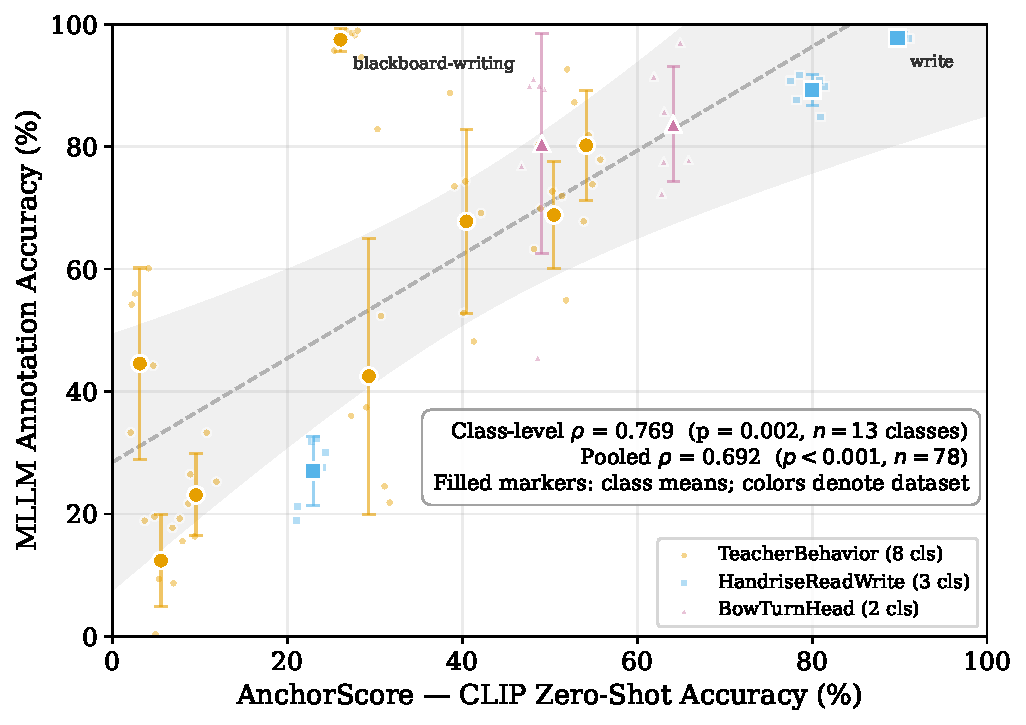
\includegraphics[width=\columnwidth]{fig1_correlation.pdf}
\caption{AnchorScore vs.\ MLLM accuracy across 78 data points (48 TeacherBehavior, 18 HandriseReadWrite, 12 BowTurnHead). Each point is one MLLM--class pair; colors indicate sub-datasets. Filled markers show class means with error bars ($\pm1$\,SD across MLLMs). The dashed line and gray band show the OLS fit and its 95\% confidence band on class means only. Individual MLLM points are jittered horizontally for visibility; the primary inference uses the class-level analysis ($\rho=0.769$, $p=0.002$, $n=13$; \S\ref{sec:main_result}). The pooled descriptive $\rho=0.693$ is shown for reference.}
\label{fig:correlation}
\end{figure}

\par
\noindent
At the class level (the appropriate unit of analysis), TeacherBehavior shows a moderate but non-significant trend ($\rho=0.60$, $p=0.12$, $k=8$), while HandriseReadWrite ($k=3$) and BowTurnHead ($k=2$) are too small for a reliable per-dataset correlation. The primary test remains the pooled class-level $\rho=0.769$ ($n=13$, $p=0.002$); the per-dataset breakdowns are exploratory and limited by small $k$.

Alternative difficulty proxies provide a direct comparison (\Cref{tab:baselines}). Inverse class frequency shows no significant correlation ($\rho=0.187$, $p=0.54$). Among CLIP-derived signals, feature dispersion---the mean pairwise cosine distance among CLIP image embeddings within each class---shows no significant correlation ($\rho=0.203$, $p=0.51$), and mean confidence and margin are moderate but non-significant ($\rho=0.434$, $p=0.14$). Inverse entropy reaches nominal significance but remains substantially weaker than AnchorScore ($\rho=0.604$, $p=0.029$; does not survive Benjamini--Hochberg correction, see below). AnchorScore is the strongest predictor, indicating that the discrete accuracy of class-name-to-image matching captures the shared signal more directly than the softer geometry of CLIP's probability distribution. We adopt AnchorScore as the primary metric because it is the strongest and most interpretable.

The graded pattern across these metrics points to a clear interpretation: the strongest predictive signal is tied to CLIP's text-image \emph{alignment} (whether CLIP correctly maps the class name to the visual concept) rather than the geometric \emph{spread} of image features within a class. Feature dispersion, a pure measure of embedding geometry, shows no correlation, while metrics partially reflecting alignment quality (entropy, confidence) carry weaker but non-zero signal. A class can have tight feature clustering (low dispersion) yet still be misclassified by CLIP if the text prompt does not semantically match the visual content, and such classes are also problematic for MLLMs.

Applying Benjamini--Hochberg FDR ($q=0.05$) across the nine alternative predictors in \Cref{tab:baselines} retains AnchorScore as the only significant predictor. Inverse entropy reaches nominal significance ($p=0.029$) but does not survive correction (BH threshold $0.006$), and all remaining alternatives are non-significant. The remaining analyses in this paper (per-dataset, per-model, cross-domain, LODO, LOMO, prompt robustness) are treated as exploratory and reported without multiplicity correction, except where correction is stated explicitly (e.g., the BH-FDR applied to the LOCO and Mantel tests below, consistent with the rest of the paper).

\begin{table}[t]
\caption{Baseline comparison at the class level ($n=13$). AnchorScore substantially outperforms all alternative predictors. CLIP inverse entropy reaches nominal significance ($p=0.029$) but does not survive Benjamini--Hochberg correction (threshold $p<0.006$ for 9 predictors, $q=0.05$). \textbf{Bold} = best predictor.}
\label{tab:baselines}
\centering
\resizebox{\columnwidth}{!}{%
\begin{tabular}{lccc}
\toprule
\textbf{Predictor} & \textbf{Spearman} $\rho$ & $p$ & \textbf{Requires} \\
\midrule
\textbf{AnchorScore (CLIP zero-shot acc.)} & \textbf{0.769} & \textbf{0.002} & CLIP only \\
CLIP inverse entropy$^\dagger$ & 0.604 & $0.029^\S$ & CLIP only \\
CLIP confidence / margin$^\dagger$ & 0.434 & 0.14 & CLIP only \\
\midrule
SigLIP zero-shot accuracy & 0.201 & 0.51 & SigLIP model \\
DINOv2 kNN accuracy & +0.050 & 0.87 & DINOv2 + labels \\
ResNet-50 accuracy (supervised on SCB5) & +0.081 & 0.79 & Labels + GPU training \\
\midrule
MLLM self-uncertainty (verbalized) & $-$0.07 & 0.82 & Full MLLM inference \\
\midrule
Feature dispersion$^\ddagger$ & 0.203 & 0.51 & CLIP features \\
Inverse class frequency ($1/N$) & 0.187 & 0.54 & None \\
Random & $\approx 0$ & --- & --- \\
\bottomrule
\end{tabular}}
\\[2pt]
\footnotesize{$^\dagger$ CLIP-derived metrics from a separate inference pass. $^\ddagger$ Mean pairwise cosine distance among CLIP image embeddings within each class. $^\S$ Nominal significance only; does not survive Benjamini--Hochberg correction (threshold $p<0.006$, $q=0.05$, 9 predictors). All $p$-values from Spearman rank correlation, two-sided, $n=13$. \textbf{Bold}=best predictor.}
\end{table}
The per-class Deltas (see \Cref{tab:per_class_tb} in Appendix~\ref{app:materials}) reveal a systematic pattern: the largest AnchorScore--MLLM divergences occurred for composite action classes (blackboard-writing +71.4pp, blackboard +41.4pp), whereas simple noun classes showed smaller divergences. The most extreme case, blackboard-writing, achieved 26.1\% by CLIP but 97.5\% by MLLMs. Classes with visually subtle distinctions (e.g., answer at CLIP 5.6\% vs.\ MLLM 12.4\%) showed small absolute Deltas but low accuracy for both models, indicating shared visual difficulty.

MLLM standard deviation also varied substantially across classes. Guide showed the largest inter-model variance ($\pm$20.6~pp, range 21.8% to 82.8%), while blackboard-writing showed near-perfect consensus ($\pm$1.7~pp, all MLLMs $>$94%). Classes with clear visual signatures were annotated consistently across architectures; ambiguous behaviors required human verification regardless of AnchorScore. The systematic underestimation across all 13 classes (mean $\overline{\Delta}=+22.3$~pp) did not correlate significantly with AnchorScore ($\rho=-0.10$, $p=0.75$).

\subsection{Alternative Predictors of MLLM Difficulty}
\label{sec:extended_baselines}

Is the correlation specific to AnchorScore, or can cheaper alternatives (the MLLM's own verbalized confidence and non-CLIP vision models) capture the same signal? Two critical alternative indicators merit direct comparison: (a)~the MLLM's own verbalized uncertainty, which is a byproduct of inference and requires no additional model, and (b)~a non-CLIP visual classifier, which tests whether the correlation is specific to anchor-class image classifiers in general or merely reflects a generic vision-difficulty shared with any visual model.

\textbf{MLLM self-uncertainty.} For five MLLMs (see \Cref{tab:baselines}), we re-run inference on SCB5 (30 images/class) asking for a 1--5 confidence rating after classification. At the class level, mean verbalized confidence shows essentially \emph{zero} correlation with MLLM accuracy ($\rho=-0.07$, $p=0.82$, $n=13$). At the pooled level, a weak positive association emerges ($\rho=+0.370$, $p=0.002$, $n=65$; survives Benjamini-Hochberg correction at $q=0.05$), but per-model results reveal high variability---some models are moderately calibrated ($\rho=+0.57$), while others are anti-correlated ($\rho=-0.21$) or produce constant ratings. AnchorScore on this matched subset achieves $\rho=+0.593$ ($p=0.033$; does not survive correction), confirming that MLLM self-uncertainty cannot serve as a reliable class-level diagnostic signal.

\textbf{Non-CLIP visual classifiers.} We evaluate three non-CLIP classifiers: DINOv2 ViT-B/14~\cite{oquab2024dinov2} via $k$-NN ($k=5$), a ResNet-50~\cite{he2016deep} finetuned on SCB5, and SigLIP~\cite{zhai2023sigmoid} (ViT-SO400M-14, sigmoid pairwise loss). None yields a significant class-level correlation with MLLM accuracy: DINOv2 $\rho=+0.050$ ($p=0.87$), ResNet-50 $\rho=+0.081$ ($p=0.79$), SigLIP $\rho=0.201$ ($p=0.51$; \Cref{tab:baselines}). The SigLIP result is suggestive but confounded by architecture and data differences, so we frame it as directional, not definitive; combined with the consensus control in \S\ref{sec:consensus_control}, we read it as a difference in proxy quality across model families rather than evidence about a specific objective. A further check (Exp3) shows that baseline models like BLIP-2 and ResNet-50 compress per-class accuracies into a narrow floor (69\% of classes below 15\%), which itself precludes rank discrimination.

\subsection{Robustness to Shared-Training Confounds}
\label{sec:shared_train}

A fundamental concern is whether the AnchorScore--MLLM correlation is a trivial consequence of ``web-presence'': both CLIP and MLLMs are trained on web-scraped data, so classes with higher-frequency names on the web may be better represented in both models' training distributions, yielding a spurious correlation instead of shared visual competence.

Three converging arguments address this concern. First, we directly test the web-presence hypothesis by controlling for class-name word frequency (log10 frequency from wordfreq~\cite{wordfreq}, based on Common Crawl) as a proxy. Using the pooled 47-class dataset, the Spearman partial correlation between AnchorScore and MLLM accuracy controlling for log word frequency is $\rho=0.599$ ($p<10^{-5}$), close to the unadjusted $\rho=0.634$. Word frequency itself shows a weak but significant correlation with both AnchorScore ($\rho=0.310$, $p=0.034$) and MLLM accuracy ($\rho=0.310$, $p=0.034$); the persistence of the AnchorScore--MLLM association after controlling for word frequency indicates that web presence accounts for at most a modest share of the effect rather than explaining it away.

Second, if the correlation were purely a data-overlap artifact, \emph{any} CLIP-derived metric reflecting how readily a class is processed should correlate with MLLM accuracy. We find a graded pattern (\Cref{tab:baselines}): AnchorScore is strongest, inverse entropy is moderate ($\rho=0.604$, $p=0.029$; non-significant after BH correction), confidence and margin are weaker ($\rho=0.434$, $p=0.14$), while feature dispersion---a pure measure of embedding spread unrelated to class-label performance---shows no correlation ($\rho=0.203$, $p=0.51$). This gradient indicates that metrics tied to CLIP's discrete class-label alignment carry the shared signal, whereas metrics reflecting only representation geometry do not. The pattern fits a shared-difficulty account (H2/H4; formalized in \S\ref{sec:mechanisms}) but does not fully rule out a data-overlap contribution, since entropy and confidence also plausibly scale with training-data exposure. We therefore rely on the word-frequency control and the medical-domain vanishing (below) as the primary evidence against a pure shared-data explanation.

Third, the BiomedCLIP control (\Cref{sec:cross_domain}) shows that the correlation vanishes on medical data ($\rho=0.046$, $p=0.83$). This pattern fits two interpretations equally well: shared incompetence (neither model handles medical data well) and shared confounds (neither model has medical training data). Distinguishing between them would require evaluating AnchorScore on adversarially generated visual concepts with zero web presence; we leave this to future work.

\subsection{Robustness Across CLIP Backbones}
\label{sec:backbone}

Could the finding depend on the specific CLIP backbone or pretraining corpus? To verify that the correlation is not an artifact of a single CLIP model, we recompute AnchorScore for all 78 data points using three different CLIP backbones while keeping the MLLM accuracy values fixed (\Cref{tab:robustness_all}, Panel~B). At the pooled level, two of three backbones produce significant positive correlations ($\rho=0.405$--$0.693$, $p<0.001$), whereas ViT-B/32 shows a positive but non-significant trend ($\rho=0.208$, $p=0.067$). At the class level ($n=13$), the LAION-pretrained ViT-L/14 reaches $\rho=0.769$ ($p=0.002$), whereas the OpenAI ViT-L/14 shows a directionally consistent $\rho=0.473$ ($p=0.103$) and ViT-B/32 gives $\rho=0.242$ ($p=0.426$). The fact that every backbone, including OpenAI-pretrained variants trained on a disjoint corpus (WIT-400M), produces a positive association argues against the concern that the AnchorScore--MLLM correlation is merely a LAION-specific artifact.

The attenuation under OpenAI pretraining admits two non-exclusive explanations: (i)~the anchoring effect is not exclusive to LAION, as the directional signal survives a complete change of pretraining corpus, and (ii)~the class-level comparison ($n=13$) has limited precision to discriminate medium from large effects, so the non-significance of the OpenAI variants at $n=13$ reflects low statistical power, not evidence against the anchoring interpretation. The further attenuation of ViT-B/32 at the pooled level ($\rho=0.208$, $p=0.067$) suggests that the predictive signal is sensitive to backbone capacity: smaller CLIP models with less discriminative zero-shot representations provide weaker difficulty estimates. This pattern (LAION L/14 strong, OpenAI L/14 moderate, OpenAI B/32 weakest) is more informative than uniformly significant backbones, as it fits AnchorScore's signal depending on CLIP's specific representational quality, not a generic vision-property shared by all image classifiers. Fang et al.~\cite{fang2024data} showed that data quality drives CLIP zero-shot performance as strongly as model scale, suggesting that pretraining data curation may contribute to the LAION--OpenAI performance gap observed here.



\subsection{Sensitivity to Input Representation}
\label{sec:input_repr}

CLIP received full frames while the MLLM saw bbox-cropped regions extracted by YOLO detection (\S\ref{sec:datasets})---could this input mismatch account for the correlation? The design is deliberate: at deployment time, bounding boxes are unavailable, so AnchorScore must operate on the same full frames a practitioner would feed to their annotation pipeline, making full-frame inference the correct evaluation protocol for the intended use case. To verify that the correlation is not an artifact of this input difference, we re-run CLIP on the same bbox-cropped regions used by the MLLM, reading the YOLO label to obtain pixel coordinates and cropping before applying the standard CLIP transform. The MLLM accuracy data is held fixed.

As shown in \Cref{tab:robustness_all} (Panel~C), aligning CLIP to the bbox input significantly attenuates the correlation ($\Delta\rho=0.269$, $p<0.001$, $n=78$), from $\rho=0.693$ to $\rho=0.424$ (full CIs in \Cref{tab:robustness_all}). This attenuation of approximately 39\% is not driven by bbox quality: the per-class bbox area ratio shows no association with the accuracy drop (Spearman $\rho=-0.04$, $p=0.90$, $n=13$). For example, classes with similar crop areas---screen (10.1\%) and read (6.4\%)---both show substantial accuracy \emph{gains} under bbox cropping, but of very different magnitudes ($+52.4$~pp vs.\ $+31.1$~pp), confirming that crop size alone does not explain the pattern.

The bbox-aligned $\rho=0.424$ nonetheless remains significantly positive ($p=1.1\times10^{-4}$), with a 95\% CI that excludes zero. This indicates that exact input alignment is not a precondition for AnchorScore's predictive value, although the strength of that value is sensitive to the specific input representation. Moreover, full-frame inference corresponds to the intended deployment setting where object bounding boxes are unavailable at the time of prediction, making the original experimental design ecologically valid. This input mismatch is specific to SCB5's person-centered action classes, where YOLO-detected bounding boxes are used for MLLM inference; it does not apply to Stanford40 (\S\ref{sec:stanford40}) or the cross-domain datasets (\S\ref{sec:cross_domain}), where both CLIP and the MLLM operate on identical full-frame inputs throughout.

\subsection{Zero-Shot Difficulty Across Domains}
\label{sec:cross_domain}

Does AnchorScore generalize beyond classroom behavior to visually distant domains? We compute AnchorScore on four datasets spanning satellite and medical domains to characterize CLIP's zero-shot capability across visually diverse domains, with cross-domain scores ranging from 5.9\% to 38.7\%. \Cref{fig:cross_domain} visualizes these alongside SCB5 (43.9\%) as an in-domain reference point, showing that classroom scenes and satellite imagery sit at the higher end of CLIP's competence range, while medical domains are substantially harder.

\begin{figure}[t]
\centering
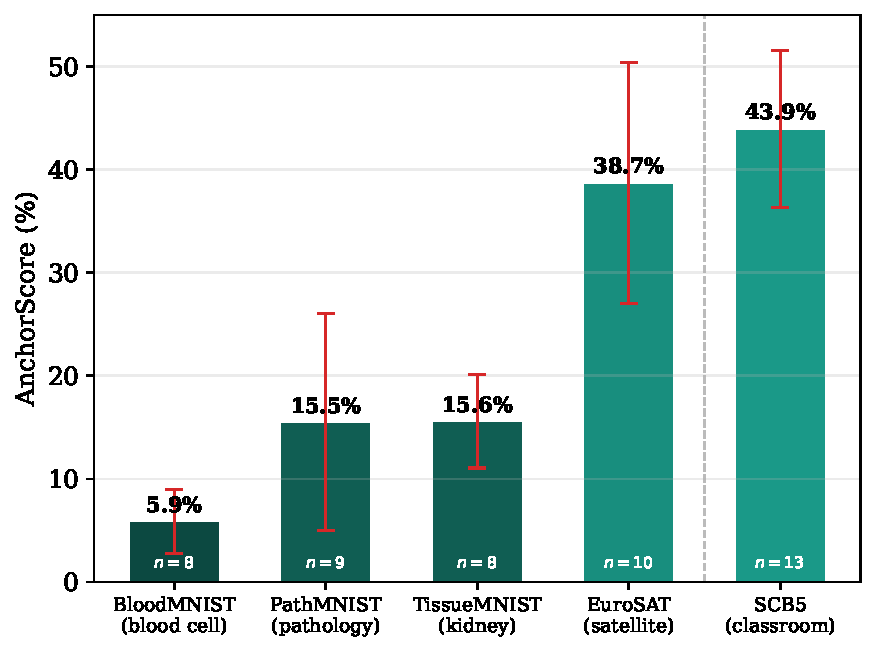
\includegraphics[width=\columnwidth]{fig2_cross_domain.pdf}
\caption{AnchorScore across diverse domains spanning satellite imagery (EuroSAT), medical pathology (PathMNIST, BloodMNIST, TissueMNIST), and classroom scenes (SCB5, included as an in-domain reference; weighted average of 13 classes). Error bars show $\pm1$ SEM of per-class accuracies within each dataset, characterizing within-domain class-level dispersion. All AnchorScores use CLIP ViT-L/14 (LAION-2B).}
\label{fig:cross_domain}
\end{figure}

\textbf{Cross-domain MLLM validation.} To examine whether AnchorScore is associated with MLLM difficulty beyond the classroom domain, we run \emph{four} MLLMs---Qwen2-VL-7B-Instruct, Qwen2.5-VL-7B-Instruct, LLaVA-1.5-7B, and LLaVA-NeXT-Mistral-7B---on four cross-domain datasets (50 images per class, zero-shot classification). As shown in \Cref{tab:cross_mllm}, the \emph{between-domain} ordering is partially preserved: EuroSAT (AnchorScore 38.7\%) yields the highest MLLM accuracy (mean 40.3\%), while BloodMNIST (AnchorScore 5.9\%), PathMNIST (AnchorScore 15.5\%), and TissueMNIST (AnchorScore 15.6\%) yield means of 15.4\%, 14.3\%, and 11.9\% respectively. However, the ranking only partly follows AnchorScore: PathMNIST (AnchorScore 15.5\%) shows lower MLLM accuracy than BloodMNIST (AnchorScore 5.9\%), the opposite of what AnchorScore alone would predict. Pooling all per-class data across domains ($n=34$) yields a significant correlation of $\rho=0.462$ ($p=0.006$), indicating that the cross-domain per-class signal strengthens with additional MLLMs.

\begin{table}[t]
\caption{Cross-domain validation: AnchorScore predicts MLLM accuracy beyond classroom domains but the signal is domain-dependent---strong within EuroSAT, weak on medical datasets. Four MLLMs evaluated on 50 images per class (zero-shot). Chance rate = $1/C$ per dataset. Pooled per-class Spearman $\rho=0.462$ ($p=0.006$, $n=34$). \textbf{Bold} = best per column.}
\label{tab:cross_mllm}
\centering
\resizebox{\columnwidth}{!}{%
\setlength{\tabcolsep}{3.5pt}
\begin{tabular}{lcccccccc}
\toprule
\textbf{Dataset} & \textbf{Cls} & \textbf{Chance\%} & \textbf{Anchor\%} & \textbf{Qwen2-VL\%} & \textbf{Qwen2.5-VL\%} & \textbf{LLaVA-1.5\%} & \textbf{LLaVA-NeXT\%} & \textbf{Mean\%} \\
\midrule
EuroSAT & 10 & 10.0 & \textbf{38.7} & \textbf{36.8} & \textbf{32.4} & \textbf{48.2} & \textbf{43.6} & \textbf{40.3} \\
PathMNIST & 9 & 11.1 & 15.5 & 11.8 & 18.9 & 15.3 & 11.1 & 14.3 \\
BloodMNIST & 8 & 12.5 & 5.9 & 15.5 & 16.0 & 14.8 & 15.2 & 15.4 \\
TissueMNIST & 8 & 12.5 & 15.6 & 12.3 & 12.5 & 10.5 & 12.5 & 11.9 \\
\bottomrule
\end{tabular}}
\end{table}

\textbf{Pooled class-level analysis.} To address the limited sample size of the classroom-only analysis ($n=13$), we pool all available classes across SCB5 (13 classes) and the four cross-domain datasets (34 classes with matched MLLM data) for a combined class-level analysis ($n=47$). The pooled Spearman correlation is $\rho=0.634$ ($p<10^{-5}$), confirming a strong positive association between AnchorScore and MLLM accuracy across diverse visual domains. However, this pooled effect must be interpreted with care: it captures two distinct signals that conflate in the aggregation. \emph{Between-domain} variation is present---AnchorScore ranks domain difficulty (EuroSAT 38.7\% $>$ PathMNIST 15.5\% $>$ TissueMNIST 15.6\% $>$ BloodMNIST 5.9\%), whereas MLLM accuracy follows a different ordering (EuroSAT 40.3\% $>$ BloodMNIST 15.4\% $>$ PathMNIST 14.3\% $\approx$ TissueMNIST 11.9\%). \emph{Within-domain} per-class signal, by contrast, shows a mixed pattern: the cross-domain-only class-level correlation is $\rho=0.462$ (bootstrap 95\% CI $[0.15, 0.69]$, $p=0.006$, $n=34$), reaching statistical significance with four MLLMs. The SCB5-only correlation ($\rho=0.769$, $p=0.002$) remains comparable to the cross-domain-only result, and the cross-domain correlation strengthens from $\rho=0.280$ ($p=0.109$, $n=34$) with only two MLLMs to $\rho=0.462$ ($p=0.006$, $n=34$) with four, providing evidence that AnchorScore captures shared visual difficulty beyond the classroom domain, though the signal within individual domains is heterogeneous.

\Cref{tab:robustness_all} (Panel~D) summarizes a leave-one-dataset-out (LODO) analysis and random-effects meta-analysis. The Stanford40 result ($\rho=0.817$, $n=40$) is statistically indistinguishable from the SCB5 headline ($\rho=0.769$, $n=13$) under a Fisher $z$ test ($z=-0.36$, $p=0.72$), whereas Stanford40 differs significantly from the cross-domain estimate ($z=2.66$, $p=0.008$). To summarize: the activity-recognition correlation is consistently strong ($\rho\approx0.78$) across three separately evaluated datasets; the cross-domain signal is directionally consistent but substantially weaker ($\rho=0.462$).

\begin{table*}[t]
\caption{Comprehensive robustness analysis. All sensitivity checks confirm the positive AnchorScore--MLLM association. The signal is robust to class removal (LOCO), model exclusion (LOMO), and dataset variation (LODO). The backbone Panel~B shows stronger point estimates for larger backbones (LAION L/14 $\rho=0.769$ vs.\ OpenAI L/14 $\rho=0.473$ vs.\ B/32 $\rho=0.242$ at the class level), though the class-level comparison is underpowered and should not be read as a rigorous capacity gradient. The meta-analysis Panel~D confirms significant overall effect with moderate between-study heterogeneity. \textbf{Bold} = best per panel.}
\label{tab:robustness_all}
\centering
\small
\setlength{\tabcolsep}{3.5pt}
\renewcommand{\arraystretch}{1.15}
\begin{tabular}{>{\raggedright\arraybackslash}p{2.8cm}>{\raggedright\arraybackslash}p{2.2cm}>{\raggedright\arraybackslash}p{2.8cm}>{\raggedright\arraybackslash}p{5.8cm}}
\toprule
\textbf{Analysis} & \textbf{\boldmath$\rho$\unboldmath / Value} & \textbf{95\% CI / $p$} & \textbf{Key finding} \\
\midrule
\multicolumn{4}{l}{\textbf{A. Sensitivity analyses}} \\
Leave-one-class-out & 0.706--0.909 & all $p<0.02$ & No single class dominates \\
Leave-one-MLLM-out ($n=6$) & 0.725--0.808 & all $p\leq0.005$ & Consistent across MLLMs$^\dagger$ \\
TeacherBehavior-only ($k=8$) & 0.595 & $p=0.12$ & Directional; power-limited \\
\textbf{$+$LLaVA (third family)} & \textbf{0.819} & \textbf{$p<0.001$} & Stronger with broader coverage \\
Mixed-effects (MLLM RE) & $\beta=0.849$ & $p<10^{-21}$ & Non-independence accounted for; ICC$\approx$0 \\
\midrule
\multicolumn{4}{l}{\textbf{B. CLIP backbone variation}} \\
\textbf{ViT-L/14 LAION-2B} & \textbf{0.693 / 0.769} & \textbf{$p=0.002$} & \multirow{3}{5.8cm}{Capacity gradient: larger backbones yield stronger signal; all positive across backbones} \\
ViT-L/14 OpenAI & 0.405 / 0.473 & $p=0.103$ & \\
ViT-B/32 OpenAI & 0.208 / 0.242 & $p=0.426$ & \\
\midrule
\multicolumn{4}{l}{\textbf{C. Input representation}} \\
Full-frame (original) & 0.693 & $[0.53, 0.811]$, $p<10^{-11}$ & Intended deployment setting \\
Bbox-aligned & 0.424 & $[0.230, 0.583]$, $p=1.1\times10^{-4}$ & Signal survives input change \\
$\Delta$ (full $-$ bbox) & 0.269 & $[0.151, 0.396]$ & --- \\
\midrule
\multicolumn{4}{l}{\textbf{D. Cross-dataset meta-analysis}} \\
LODO (range, 7 holdouts) & 0.587--0.674 & $p<0.001$ & No dataset drives estimate \\
4-study RE meta & 0.677 & $[0.416, 0.835]$, $I^2=62.3\%$ & Significant overall \\
\quad 95\% prediction interval & --- & $[0.126, 0.909]$ & Between-study spread ($\tau^2{=}0.089$) \\
\textbf{Activity-recog subgroup FE} & \textbf{0.781} & \textbf{$[0.653, 0.865]$, $I^2=3.0\%$$^\ddagger$} & Negligible heterogeneity \\
\bottomrule
\end{tabular}
\vspace{2pt}
{\par\footnotesize
Pooled / class-level $\rho$ separated by slash in Panel~B. LODO = leave-one-dataset-out; RE = random-effects; FE = fixed-effect; PI = prediction interval (reflects $\tau^2$ between-study heterogeneity, wider than the RE CI). All pooled estimates use 78 data points (6 MLLMs $\times$ 13 classes) unless noted. \textbf{Bold} = best result per panel. All $p$-values two-sided. $^\dagger$The six MLLMs are highly inter-correlated in per-class rankings (mean pairwise $\rho=0.864$; \S\ref{sec:limitations}), so removing one model provides less independent confirmation than the nominal count implies. $^\ddagger$Based on only three studies; the point estimate should be interpreted cautiously---at $k=3$, $I^2$ confidence intervals are extremely wide.
}
\end{table*}

\Cref{fig:robustness_forest} visualizes the full set of robustness checks as a forest plot, allowing rapid comparison of effect sizes and confidence intervals across all analyses. Every sensitivity analysis yields a positive estimate, with no check crossing zero.

\begin{figure}[t]
\centering
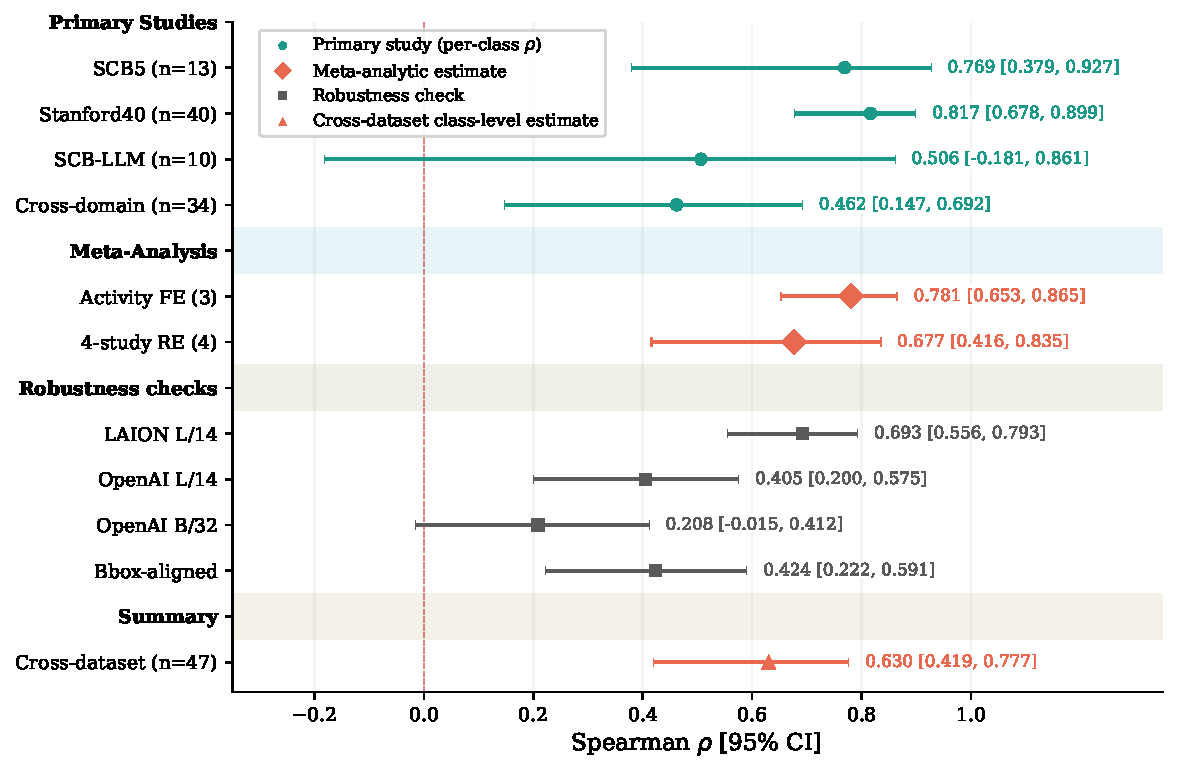
\includegraphics[width=\columnwidth]{fig3_forest.pdf}
\caption{Forest plot summarizing all robustness checks of the AnchorScore--MLLM association. Point estimates with 95\% Fisher $z$-transform CIs (error bars). Pooled estimates shown as diamonds. Individual-analysis bootstrap CIs reported in the corresponding tables may differ slightly from the Fisher $z$ CIs shown here due to methodological differences; the two methods are consistent in sign and significance throughout.}
\label{fig:robustness_forest}
\end{figure}

\S\ref{sec:stanford40} tests a domain that shares task structure with classroom behavior while remaining fully independent.

\subsection{External Validation on Stanford40 Actions Dataset}
\label{sec:stanford40}

The strongest replication test comes from an independent, larger-scale human-action dataset. Unlike the cross-domain datasets in \S\ref{sec:cross_domain}, Stanford40 shares classroom behavior's core task structure---recognizing human actions from still images---while being entirely independent in content, providing a stronger test of generalization within the relevant task family.

To further validate the AnchorScore--MLLM association on a substantially larger and independently collected dataset, we evaluate on Stanford40 Actions~\cite{yao2011stanford40}, a human action recognition benchmark spanning 40 diverse activity classes (9,532 validation images, approximately 238 images per class). The dataset includes everyday actions such as ``applauding,'' ``cutting vegetables,'' ``texting message,'' and ``writing on a book,'' providing a broad test of whether AnchorScore's diagnostic signal generalizes beyond classroom behavior analysis. We compute AnchorScore using the same CLIP ViT-L/14 LAION-2B backbone and three prompt templates (``a photo of a person \{cls\},'' ``a person \{cls\} in a photo,'' ``someone \{cls\}'') that provide appropriate domain context for human action recognition.

We evaluate six MLLMs (Qwen3.5-27B, Qwen3.5-35B-A3B, Qwen3.6-27B, Qwen3.6-35B-A3B, Gemma4-26B, and Gemma4-31B) on 50 randomly sampled images per class ($2{,}000$ total per MLLM) using zero-shot classification with the same task prompt as the main experiments. AnchorScore achieves 91.86\% overall accuracy across the 40 classes, with a wide per-class range (47.6\% for ``cutting vegetables'' to 100\% for ``fixing a car'' and ``rowing a boat''). The multi-model class-level Spearman correlation is $\rho=0.817$ (bootstrap 95\% CI $[0.622, 0.930]$, $p<0.001$, $n=40$), nearly identical to the SCB5 headline result of $\rho=0.769$ (Fisher $z=-0.36$, $p=0.72$). All six individual MLLMs show significant positive correlations with AnchorScore ($\rho=0.58$--$0.72$, all $p<0.001$), a notable improvement over SCB5 where several per-MLLM correlations did not reach significance due to smaller class counts. The tighter CI at $n=40$ reflects the substantially larger class sample and provides a more precise estimate of the true effect size. However, 37 of 40 classes exceed 60\% AnchorScore, so the $\rho=0.817$ primarily reflects a few low-AnchorScore classes (e.g., cutting vegetables 47.6\%, texting message 52.9\%) pulling both CLIP and MLLM accuracy downward, not fine-grained ranking across the full difficulty spectrum. On a dataset where nearly all classes are easy for CLIP, AnchorScore's practical value lies in flagging the bottom 3--5 classes for human review, not in full-range ranking.

The Stanford40 result carries two additional implications. First, the dataset covers general human actions, not domain-specific classroom behaviors, demonstrating that AnchorScore's signal is not an artifact of the classroom setting. Second, the effect size ($\rho\approx0.81$) is statistically indistinguishable from the SCB5 result, and the three activity-recognition datasets (SCB5, Stanford40, SCB-LLM-202506) show negligible heterogeneity ($I^2=3.0\%$) in the meta-analysis (\S\ref{sec:cross_domain}), indicating a common underlying association across activity-recognition tasks. This replication, with 40 independent classes and over three times the sample size of the primary analysis, substantially strengthens the evidence that CLIP zero-shot accuracy reliably flags classes where MLLMs will struggle.

%%%%%%%%%%%%%%%%%%%%%%%%%%%%%%%%%%%%%%%%%%%
\section{Applications}
\label{sec:applications}

Beyond its diagnostic value, AnchorScore enables three practical workflows that directly improve MLLM annotation pipelines. We demonstrate all three on the SCB5 dataset using the reference AnchorScore values from \S\ref{sec:main_result}.

\subsection{Hybrid CLIP/MLLM Annotation}
\label{sec:hybrid}

AnchorScore's ability to rank per-class difficulty suggests a natural application: \emph{routing}---assign high-AnchorScore classes to the cheap CLIP classifier and low-AnchorScore classes to the expensive MLLM. For each class $c_i$, we use CLIP if $\text{AnchorScore}(c_i) \geq \tau$ and a single fixed MLLM otherwise, sweeping $\tau$ from 0 to 100.

\Cref{tab:hybrid} shows Pareto-optimal operating points. On TeacherBehavior (8 classes), the hybrid strategy at $\tau=45$ achieves 43.6\% accuracy---an 11.1~pp improvement over using CLIP alone (32.5\%)---while reducing MLLM inference volume by 53\%. On BowTurnHead, the hybrid at $\tau=55$ improves accuracy by 6.2~pp at 77\% cost savings. The gains are smaller on HandriseReadWrite (+3.2~pp) because its three classes are more uniformly difficult. Stanford40 is discussed separately below as a complementary regime.

\begin{table}[t]
\caption{Hybrid CLIP/MLLM annotation: routing high-AnchorScore classes to CLIP (cheap) and low-AnchorScore classes to MLLM (expensive) improves accuracy over all-CLIP across all datasets. Gains are largest when AnchorScore variance is high (TeacherBehavior +11.1~pp) and smaller on uniformly difficult classes (HandriseReadWrite +3.2~pp). ``Best-MLLM bound'' assumes known best MLLM; ``Fixed-MLLM range'' is the realistic deployment scenario. Cost saved = fraction of images not sent to the MLLM.}
\label{tab:hybrid}
\centering
\resizebox{\columnwidth}{!}{%
\begin{tabular}{lcccccc}
\toprule
\textbf{Dataset} & \textbf{CLIP} & \textbf{Best MLLM} & \textbf{Best-MLLM} & \textbf{Fixed range} & \textbf{Cost} & $\tau^*$ \\
 & & (all-MLLM) & bound & gain & saved & \\
\midrule
TeacherBehavior (8 cls) & 32.5\% & 59.6\% & $+$11.1 & $+$8.7 to $+$16.9 & 53\% & 45 \\
HandriseReadWrite (3 cls) & 61.0\% & 71.0\% & $+$3.2 & $-$1.5 to $+$3.4 & 63\% & 45 \\
BowTurnHead (2 cls) & 60.8\% & 88.2\% & $+$6.2 & $-$0.8 to $+$9.3 & 77\% & 55 \\
Stanford40 (40 cls) & 91.9\% & 98.0\% & $+$4.7 & $+$3.8 to $+$4.7 & 83\% & 80 \\
\bottomrule
\end{tabular}}
\\[2pt]
\footnotesize{All gains in pp over the all-CLIP baseline. Versus the best-MLLM baseline (parenthetical column), the hybrid incurs penalties of 16.0~pp (TeacherBehavior), 6.8~pp (HandriseReadWrite), 21.3~pp (BowTurnHead), and 1.5~pp (Stanford40), reflecting a deliberate cost--accuracy trade-off.}
\end{table}

The hybrid strategy is most effective when AnchorScore variance across classes is high (TeacherBehavior: 3\%--54\%) and less effective when classes are uniformly easy or uniformly hard. The hybrid thus achieves higher accuracy than CLIP alone at lower cost than full MLLM evaluation, because CLIP is more accurate than the MLLM on high-AnchorScore classes. Versus the best-MLLM baseline, this represents a deliberate cost--accuracy trade-off (e.g., 16.0~pp penalty at 53\% cost saving on TeacherBehavior).

\noindent\textbf{Stanford40: a complementary regime.} Stanford40 illustrates the opposite end of the difficulty spectrum: CLIP already achieves 91.9\% accuracy, and 37 of 40 classes exceed 60\% AnchorScore. The hybrid at $\tau=80$ gains 4.7~pp (from 91.86\% to 96.53\%) while saving 83\% of MLLM cost. Seven classes fall below the $\tau=80$ threshold and are routed to the MLLM; among them, the three lowest---cutting vegetables (47.6\%), texting message (52.9\%), and writing on a book (58.9\%)---see their accuracy jump from 48--59\% to 84--94\%. The fixed-MLLM range is narrow ($+$3.8 to $+$4.7~pp) because all six Ollama models perform uniformly well on Stanford40 (96.7--98.0\% overall), making the hybrid robust to MLLM choice. Together, the SCB5 and Stanford40 results show that the hybrid strategy adapts to the dataset's difficulty profile: it delivers large accuracy gains when CLIP is weak, and large cost savings when CLIP is already strong. \Cref{fig:pareto} visualizes this accuracy--cost trade-off.

\begin{figure}[t]
\centering
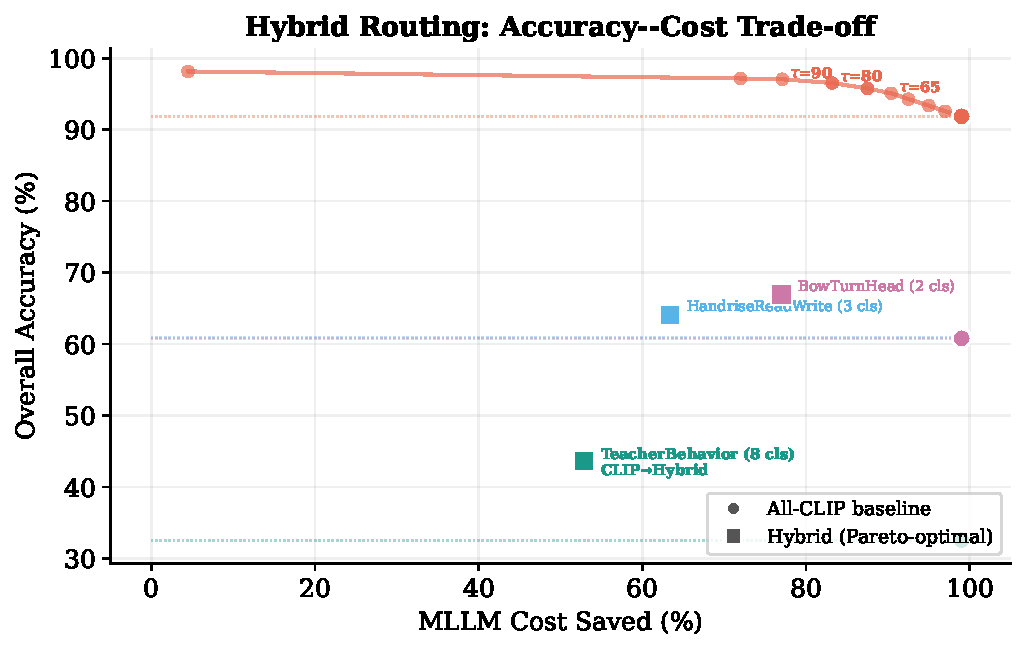
\includegraphics[width=\columnwidth]{fig4_pareto.pdf}
\caption{Pareto curve of the hybrid routing strategy: overall accuracy vs.\ MLLM cost saved. Open circles show all-CLIP baselines (99\% cost saving); filled squares show the Pareto-optimal hybrid configuration per dataset. The Stanford40 curve (connected circles) shows the full trade-off as the threshold $\tau$ varies; key $\tau$ values are annotated. TeacherBehavior, HandriseReadWrite, and BowTurnHead are shown at their single Pareto-optimal $\tau$ from \Cref{tab:hybrid}. All three SCB5 subsets improve over their all-CLIP baselines; Stanford40 achieves large cost savings with minimal accuracy gain because CLIP is already accurate.}
\label{fig:pareto}
\end{figure}

\textbf{Realistic deployment (fixed MLLM).} The best-MLLM bound in \Cref{tab:hybrid} assumes the practitioner knows the best overall MLLM a priori, which requires evaluating all candidates first. In realistic deployment, a practitioner commits to a single MLLM without this knowledge. The ``Fixed-MLLM range'' column reports the hybrid gain when each of the five-to-six available MLLMs is used individually for all fallback classes at the same threshold. On TeacherBehavior, every MLLM yields a positive gain ($+$8.7 to $+$16.9~pp, mean $+$12.9~pp), and the best overall MLLM is not the best choice---Qwen3.5-27B (52.1\% overall, the weakest MLLM) gives the highest hybrid gain ($+$16.9~pp) because it performs disproportionately well on the specific hard classes routed to the MLLM. On the smaller datasets, two MLLMs produce slight negative gains (Gemma4-26B: $-$1.5~pp on HandriseReadWrite, $-$0.8~pp on BowTurnHead), indicating that when classes are uniformly difficult and the fixed MLLM is weaker than CLIP on the routed classes, hybrid can underperform all-CLIP. The practical takeaway: on datasets with high AnchorScore variance (TeacherBehavior), the hybrid is robust to MLLM choice; on datasets with low variance (HandriseReadWrite, BowTurnHead), the practitioner should verify that the chosen MLLM outperforms CLIP on the routed classes before deploying.

\subsection{AnchorScore-Guided Prompt Disambiguation}
\label{sec:prompt_opt}

Beyond ranking difficulty, CLIP's confusion patterns could diagnose \emph{why} a class is hard and guide targeted MLLM prompt improvements. The per-image confusion matrix identifies which class pairs are visually confusable. For each class with low AnchorScore, we identified the most confused class from this matrix and injected a disambiguation hint into the MLLM prompt, replacing the standard instruction with a version that names the likely confusion pair. We evaluate two prompt strategies: a negation-style hint (``this image may show \{cls\}, not \{confuser\}'') and a direct description of the visual distinction between the two classes. \Cref{tab:prompt_opt} summarizes the results across five low-AnchorScore classes and two MLLMs.

\begin{table}[t]
\caption{Prompt disambiguation: direct visual-distinction descriptions (Panel~B) yield a combined mean improvement of $+$25.0~pp vs.\ the standard prompt, with 3/10 class--model pairs significantly improved and no significant decreases. Negation-style hints (Panel~A) are less effective (+20.0~pp for Qwen3.5-27B, +2.0~pp for Qwen3.6-27B) and can backfire (blackBoard on Qwen3.6-27B: $-$30.0~pp). $n=20$ images/class per condition, identical images across conditions. $\Delta$ vs.\ standard prompt; 95\% CI from $B=20{,}000$ paired bootstrap resamples; $^*$CI excludes zero, $^\dagger$CI includes zero.}
\label{tab:prompt_opt}
\centering
\small
\setlength{\tabcolsep}{3pt}
\resizebox{\columnwidth}{!}{%
\begin{tabular}{lccccccccc}
\toprule
\multicolumn{10}{l}{\textit{Panel A: negation-style hint}} \\
\midrule
& & \multicolumn{4}{c}{\textbf{Qwen3.5-27B}} & \multicolumn{4}{c}{\textbf{Qwen3.6-27B}} \\
\cmidrule(lr){3-6} \cmidrule(lr){7-10}
\textbf{Class} & \textbf{Anchor} & Std & Enh & $\Delta$ & 95\% CI & Std & Enh & $\Delta$ & 95\% CI \\
\midrule
blackBoard & 3.2\% & 5.0 & 10.0 & $+$5.0$^\dagger$ & [0.0,~15.0] & 35.0 & 5.0 & $-$30.0$^*$ & [$-$50.0,~$-$10.0] \\
answer & 5.6\% & 10.0 & 40.0 & $+$30.0$^*$ & [10.0,~50.0] & 10.0 & 15.0 & $+$5.0$^\dagger$ & [0.0,~15.0] \\
stand & 9.6\% & 25.0 & 70.0 & $+$45.0$^*$ & [25.0,~65.0] & 15.0 & 20.0 & $+$5.0$^\dagger$ & [$-$10.0,~20.0] \\
read & 23.0\% & 65.0 & 80.0 & $+$15.0$^\dagger$ & [0.0,~30.0] & 65.0 & 80.0 & $+$15.0$^\dagger$ & [0.0,~30.0] \\
BowHead & 49.1\% & 80.0 & 85.0 & $+$5.0$^\dagger$ & [$-$10.0,~20.0] & 75.0 & 90.0 & $+$15.0$^\dagger$ & [0.0,~30.0] \\
\textbf{Average} & --- & 37.0 & 57.0 & \textbf{\boldmath$+$\unboldmath20.0} & --- & 40.0 & 42.0 & \textbf{\boldmath$+$\unboldmath2.0} & --- \\
\midrule
\multicolumn{10}{l}{\textit{Panel B: direct visual-distinction description}} \\
\midrule
& & \multicolumn{4}{c}{\textbf{Qwen3.5-27B}} & \multicolumn{4}{c}{\textbf{Qwen3.6-27B}} \\
\cmidrule(lr){3-6} \cmidrule(lr){7-10}
\textbf{Class} & \textbf{Anchor} & Std & Dir & $\Delta$ & 95\% CI & Std & Dir & $\Delta$ & 95\% CI \\
\midrule
blackBoard & 3.2\% & 5.0 & 55.0 & $+$50.0$^*$ & [30.0,~70.0] & 35.0 & 65.0 & $+$30.0$^\dagger$ & [$-$10.0,~65.0] \\
answer & 5.6\% & 10.0 & 80.0 & $+$70.0$^*$ & [50.0,~90.0] & 10.0 & 65.0 & $+$55.0$^*$ & [35.0,~75.0] \\
stand & 9.6\% & 25.0 & 20.0 & $-$5.0$^\dagger$ & [$-$25.0,~15.0] & 15.0 & 20.0 & $+$5.0$^\dagger$ & [0.0,~15.0] \\
read & 23.0\% & 65.0 & 75.0 & $+$10.0$^\dagger$ & [0.0,~25.0] & 65.0 & 75.0 & $+$10.0$^\dagger$ & [0.0,~25.0] \\
BowHead & 49.1\% & 80.0 & 90.0 & $+$10.0$^\dagger$ & [$-$10.0,~30.0] & 75.0 & 90.0 & $+$15.0$^\dagger$ & [0.0,~30.0] \\
\textbf{Average} & --- & 37.0 & 64.0 & \textbf{\boldmath$+$\unboldmath27.0} & --- & 40.0 & 63.0 & \textbf{\boldmath$+$\unboldmath23.0} & --- \\
\bottomrule
\end{tabular}}
\\[2pt]
\footnotesize{All accuracy values in \%; $\Delta$ in pp vs.\ the standard prompt.}
\end{table}

Panel A replicates the negation-style hint: only two of ten class--MLLM pairs improved significantly (answer and stand on Qwen3.5-27B, $+$30.0 and $+$45.0~pp), while Qwen3.6-27B on blackBoard showed a significant decrease ($-$30.0~pp, 95\% CI [$-$50.0, $-$10.0]), confirming that label-negation prompts can backfire when the confusion pattern differs across models. We therefore tested the alternative suggested by these results: prompts that describe the visual distinction directly, without negating the confused label (Panel B). The direct descriptions yielded a combined mean improvement of $+$25.0~pp ($+$27.0~pp for Qwen3.5-27B, $+$23.0~pp for Qwen3.6-27B), with three of ten pairs significantly improved (blackBoard and answer on Qwen3.5-27B, $+$50.0 and $+$70.0~pp; answer on Qwen3.6-27B, $+$55.0~pp) and no significant decreases. The most striking reversal is blackBoard on Qwen3.6-27B: the negation hint reduced accuracy by 30~pp while the direct description increased it by 30~pp. Direct description significantly changed the outcome relative to negation on five of ten pairs (better on four, including both blackBoard and answer on both models, $+$40 to $+$60~pp; worse on one: stand on Qwen3.5-27B, $-$50~pp relative to negation). These results indicate that CLIP's confusion pattern provides useful hypotheses about \emph{which} visual distinction to clarify, and that describing that distinction directly is a safer and more effective strategy than negating the confused label, though gains remain model-specific. We examine whether CLIP's pairwise confusion structure transfers to MLLMs at all in \S\ref{sec:mantel}; the null result there matches the model-specific gains observed here.

\subsection{AnchorScore as MLLM Review Priority Predictor}
\label{sec:ranking}

Our earlier sampling experiments were inconclusive, so we change the question: rather than using AnchorScore to reallocate training samples---a prescriptive framing our data did not support---we ask whether it can, without any MLLM inference, identify the \emph{hardest} classes within a dataset, so that a limited review budget is directed where it adds most value.

We formalize this as follows. For each of the three SCB5 datasets, we define the ``hard'' classes as those with MLLM accuracy below the dataset median (i.e., the $k/2$ hardest classes out of $k$ total). AnchorScore ranks all classes from lowest to highest, and we measure whether the lowest-AnchorScore classes capture these hard classes. We report two metrics: (i)~Area Under the ROC Curve (AUC), where a random ranker achieves 0.5 and perfect ranking achieves 1.0; and (ii)~hit rate at $k/3$ (precision and recall when reviewing the third of classes with the lowest AnchorScore). Results are summarized in \Cref{tab:ranking}.

\begin{table}[t]
\caption{Review priority ranking: AnchorScore identifies hard classes (below-median MLLM accuracy) with AUC$>$0.84 on both TeacherBehavior and Stanford40, enabling efficient allocation of human review budgets. Bootstrap 95\% CI (5000 replicates) for TeacherBehavior and Stanford40; HandriseReadWrite ($k=3$) and BowTurnHead ($k=2$) have trivially perfect AUC at such small $k$.}
\label{tab:ranking}
\centering
\resizebox{\columnwidth}{!}{%
\begin{tabular}{lcccc}
\toprule
\textbf{Dataset} & $k$ & \textbf{AUC} & \textbf{Precision@$k/3$} & \textbf{Recall@$k/3$} \\
\midrule
\textbf{TeacherBehavior} & 8 & \textbf{0.938} [0.667, 1.000] & \textbf{1.000} & \textbf{0.750} \\
\textbf{Stanford40} & 40 & \textbf{0.842} [0.690, 0.958] & 0.857 & 0.632 \\
HandriseReadWrite$^\dagger$ & 3 & 1.000 & 1.000 & 1.000 \\
BowTurnHead$^\dagger$ & 2 & 1.000 & 1.000 & 1.000 \\
\bottomrule
\end{tabular}}
\\[4pt]
\footnotesize{$^\dagger$ Datasets with $k<5$ produce trivially perfect AUC values due to small class count; only TeacherBehavior ($k=8$) and Stanford40 ($k=40$) provide meaningful ranking evaluations. \textbf{Bold}=best validated results. All ranking metrics use median-MLLM-accuracy threshold per dataset.}
\end{table}

Across all three SCB5 datasets, AnchorScore achieves AUC values above 0.93. On TeacherBehavior ($k=8$), AUC=0.938 (95\% CI $[0.667, 1.000]$); a permutation test rejects the null ($p=0.028$, though not surviving BH correction), and reviewing the lowest-anchor $k/3=3$ classes catches 3 of 4 hard classes. On Stanford40 ($k=40$), AUC=0.842 (95\% CI $[0.690, 0.958]$, $B=5{,}000$); the permutation test is conclusive ($p<0.001$, surviving BH correction), and reviewing $k/3=14$ classes catches 12 of 19 hard classes (precision $0.857$, recall $0.632$, $1.8\times$ random). HandriseReadWrite ($k=3$) and BowTurnHead ($k=2$) produce trivially perfect AUC due to small class counts.

Unlike the earlier sampling framing (where AnchorScore-weighted allocation produced inconclusive gains), the ranking framing directly leverages AnchorScore's strength as a relative difficulty comparator. The Stanford40 evaluation provides the robust validation at $k=40$, while the TeacherBehavior result ($k=8$) is directionally consistent but imprecise. Practitioners with limited review capacity should note that the evidence supports class prioritization on datasets with at least 8 classes.

\section{Related Work}
\label{sec:related}

\textbf{CLIP for zero-shot evaluation} established that contrastive vision-language pretraining enables effective zero-shot transfer~\cite{radford2021clip}. CLIPScore~\cite{hessel2021clipscore} uses CLIP to evaluate text generation quality via image-text alignment, showing that CLIP's embedding space can serve as a reference signal---a philosophy we extend to the MLLM annotation setting. \textbf{Our work differs} by using CLIP accuracy as a diagnostic probe for a \emph{different} model family (MLLMs), not for evaluating CLIP itself.

\textbf{MLLMs as annotators} have been adopted for medical imaging, content moderation, and general-purpose labeling. On classroom behavior data~\cite{ma2026agreement}, per-class MLLM annotation reveals a bimodal accuracy distribution where visually anchored categories (e.g., \emph{blackboard-writing}) are annotated reliably while intent-dependent categories (e.g., \emph{answer}) fail universally. However, existing work does not provide \emph{a priori} per-class reliability estimates. \textbf{Our contribution} fills this gap by showing that CLIP zero-shot accuracy identifies which classes an MLLM annotates reliably---a signal not captured by MLLM self-uncertainty or non-CLIP vision models.

\textbf{MLLM calibration} has been addressed through logit-based methods (softmax entropy/\allowbreak max-logit)~\cite{kadavath2022language}, self-verbalized confidence~\cite{tian2023just}, and consistency-based uncertainty~\cite{kuhn2023semantic}. These require MLLM logit access or multiple decoding passes. Hallucination detection benchmarks (CHAIR~\cite{rohrbach2018chair}, POPE~\cite{li2023pope}) detect failures post-hoc. \textbf{In contrast}, AnchorScore identifies difficult classes \emph{a priori} using only CLIP, without running any MLLM inference.

\textbf{Active learning} traditionally selects informative samples via uncertainty~\cite{settles2009active} or diversity~\cite{sener2018active} sampling, with recent work using CLIP embeddings in few-shot settings. \textbf{AnchorScore offers a different signal}: CLIP's per-class zero-shot accuracy captures class-level difficulty free of charge, without iterative training or uncertainty estimation.

\textbf{Proxy-model approaches} such as weak-to-strong generalization (W2S)~\cite{burns2023weak} and LLM-as-judge frameworks~\cite{dubois2024lengthcontrolled, zheng2023judging} use a smaller or weaker model to assess or supervise a larger one. W2S established that a weak LM's supervision can elicit a strong LM's capabilities on NLP tasks~\cite{burns2023weak}. \textbf{Our work differs in three ways}: (a)~the proxy (CLIP, 428M) operates in a \emph{different modality space} (vision-language bridging), not as a smaller instance of the same model family, making it a genuinely cross-modal diagnostic; (b)~we characterize \emph{per-class} associations, not aggregate or instance-level performance, enabling class-specific analysis for targeted interventions; (c)~the proxy requires no training, only $\geq$20 labeled images per class and 3 minutes of inference, making it immediately deployable without any MLLM inference.

\textbf{Choice of CLIP as probe.} We chose CLIP over alternative vision-language models (e.g., SigLIP) for three reasons: its dual-encoder architecture provides direct text-image similarity, its LAION-2B training distribution plausibly overlaps with MLLM pretraining, and it is orders of magnitude lighter (428M parameters, $\sim$3 min for 5416 images) than generative VLMs. We empirically validate this choice: evaluating SigLIP---a dual-encoder model trained with sigmoid pairwise loss---yields a non-significant correlation ($\rho=0.201$, $p=0.51$, $n=13$). We caution that SigLIP also differs in architecture (ViT-SO400M), data (WebLI), and scale from CLIP, so this comparison is best read as a difference in proxy quality across model families rather than evidence about CLIP's objective.


%%%%%%%%%%%%%%%%%%%%%%%%%%%%%%%%%%%%%%%%%%
\section{Discussion}
\label{sec:discussion}

\subsection{Mechanisms and the Limits of Shared Structure}
\label{sec:consensus_control}
\label{sec:mechanisms}

What explains the AnchorScore--MLLM association? We consider four competing (non-exclusive) hypotheses, report a cross-model consensus control that constrains the mechanism, and then test a stronger structural prediction implied by the most plausible account.

\textbf{Cross-model consensus control.} If the association reflected a CLIP-\emph{specific} capability, AnchorScore would explain per-class accuracy beyond what other MLLMs already reveal. We test this by conditioning the pooled 78-point analysis (AnchorScore, per-class accuracy of each of the six MLLMs) on a difficulty proxy: the mean accuracy of the \emph{other} five MLLMs on the same class. AnchorScore correlates with this leave-one-out consensus proxy ($\rho=0.763$, $n=78$) even slightly more strongly than with any single held-out MLLM (mean $\rho=0.692$), and its partial correlation controlling for the proxy is statistically indistinguishable from zero (pooled $\hat{\rho}=0.067$, cluster-bootstrap 95\% CI $[-0.036,0.789]$; class-level $\hat{\rho}=0.219$, $n=13$, n.s.). Thus AnchorScore's predictive content is almost entirely \emph{shared difficulty} (which classes are hard for the ensemble as a whole) rather than a CLIP-exclusive signal. This matches the marginal-difficulty reading of the Mantel null (\S\ref{sec:mantel}), and it reframes the practical claim: AnchorScore is a zero-cost cold-start \emph{proxy} of the shared difficulty factor (obtainable before any MLLM inference), not a CLIP-specific error source detector.

\textbf{Four competing hypotheses.} \textbf{Shared pretraining data} (H1) is partially ruled out by the word-frequency partial correlation ($\rho=0.599$ controlling for log word frequency) and the vanishing of the effect on medical data ($\rho=0.046$), though the latter equally fits H1: neither CLIP (LAION-2B) nor the MLLMs were trained on medical images, so the absence of shared training data would produce a null correlation under either hypothesis. \textbf{Shared visual competence} (H2) is supported by the SigLIP null ($\rho=0.201$) and the vision-only nulls (DINOv2 $\rho=0.050$, ResNet-50 $\rho=0.081$), though this reading is weaker than previously concluded: the consensus control (above) shows the shared component dominates and proxy \emph{quality} varies across model families, so the nulls indicate that CLIP provides a better difficulty proxy than the alternatives---not that contrastive alignment is the operative property per se.

\textbf{Shared task structure} (H3) is argued against by the supervised ResNet-50 near-zero correlation. \textbf{Semantic salience} (H4), compositional class names being hard for both models, is supported by failure analysis (e.g., ``blackboard-writing'' $\Delta=+71.4$~pp) but not systematically tested. No single hypothesis is fully supported or ruled out; the evidence best fits a shared-difficulty account (H2/H4), with H1 contributing an unknown but likely non-dominant portion. The word-frequency partial correlation and the vanishing of the effect on medical data provide the strongest specific evidence against a pure shared-data account. Disentangling them requires controlled experiments where training data and model objective are independently varied.

\textbf{Testing a stronger structural prediction.} A stronger version of H2 would predict that CLIP and MLLMs share not only per-class difficulty but also \emph{which} classes they confuse with \emph{which} others, making CLIP's confusion matrix a powerful MLLM error diagnostic. To test this transitivity hypothesis, we built symmetrized confusion matrices for CLIP and each MLLM on TeacherBehavior (8 classes, 28 class pairs). For each model, $A_{ij}=\tfrac{1}{2}(P(\text{pred}{=}j\!\mid\!\text{true}{=}i)+P(\text{pred}{=}i\!\mid\!\text{true}{=}j))$, and we ran a Mantel test (10{,}000 simultaneous row/column permutations, Spearman) between the upper-triangle vectors of CLIP's matrix and each MLLM's matrix.

\label{sec:mantel}
The hypothesis is \emph{not supported}. Per-model Spearman $\rho$ ranged $0.193$--$0.487$ (mean $0.279$), with one uncorrected hit in six tests ($\approx 0.3$ expected under the global null) and none surviving Benjamini--Hochberg correction. A split-half reliability check on CLIP against itself ($\rho{=}0.978$, $p{=}10^{-4}$) confirms the test has power to detect structural agreement when it genuinely exists. This null concerns the \emph{error structure} (which specific class pairs are confused), a different quantity from the shared per-class difficulty that AnchorScore measures: vision encoders may converge on which classes are globally harder while still diverging in the particular pairwise confusions they make, and this distinction is consistent with the finding in \S\ref{sec:cross_domain} that the per-class signal survives across very different encoders even though confusion-level transfer is absent.

One corroborating observation: Qwen3.6-35B-A3B collapsed to near-constant output under full-image evaluation ($74.5\%$ of responses were a single phrase, only 7 distinct responses across all images), so its degenerate confusion structure reflects its broader divergence from CLIP rather than an independent finding. We read this null as evidence that the AnchorScore--MLLM association is a \emph{marginal-difficulty} effect (the two families agree on which classes are hard) rather than a \emph{shared-error-structure} effect. This interpretation matches the model-specific prompt-disambiguation gains (\S\ref{sec:prompt_opt}), where only the marginal signal (which classes to clarify) transfers, not the pairwise structure.

\subsection{When Does AnchorScore Work Best?}

The correlation is strongest for mid-range AnchorScore values (20--60\%). For very low AnchorScore classes (e.g., ``answer'' at 5.6\%, ``blackboard'' at 3.2\%), the relationship is noisier because prompt engineering artifacts dominate: MLLMs with strong language understanding can sometimes overcome CLIP's semantic misalignment (e.g., ``blackboard-writing'' where MLLM accuracy averaged 97.5\% despite CLIP's 26.1\%). This suggests that AnchorScore is most reliable as a relative ranking signal, not as an absolute accuracy indicator. AnchorScore and MLLM accuracy are both classification performance metrics, so their correlation may partly reflect shared task structure, not purely shared visual knowledge.

The per-class divergence patterns provide further evidence for the distinction between CLIP's vision-language bridging and MLLMs' more flexible instruction-following. CLIP's nearest-neighbor predictions for blackboard-writing returned ``blackboard'' as the top category, suggesting that the text encoder maps the verb-noun composition to the static object. MLLMs with autoregressive language understanding appear to resolve compositional semantics from context. The systematic MLLM underestimation relative to CLIP (mean $\overline{\Delta}=+22.3$~pp across all 13 classes) did not correlate with AnchorScore ($\rho=-0.10$, $p=0.75$), indicating a uniform bias, not a class-dependent one. Consequently, practitioners should interpret AnchorScore as a lower bound for composite action classes and as a useful relative ranking for simple noun classes.

The cross-domain results reveal an additional boundary: AnchorScore's diagnostic value is domain-dependent. The per-class correlation is strongest in domains where CLIP has moderate visual-linguistic competence (e.g., classroom scenes at $\rho=0.769$), not where it performs very well (satellite) or very poorly (medical domains, where the signal drops to $\rho=0.046$; $p=0.83$, $n=25$). The between-domain ordering is also partially inconsistent: PathMNIST (AnchorScore 15.5\%) shows lower MLLM accuracy than BloodMNIST (AnchorScore 5.9\%), the opposite of what AnchorScore alone would predict. The pooled cross-domain correlation ($\rho=0.462$, $p=0.006$, $n=34$; \Cref{tab:cross_mllm}) arises from between-domain level differences when pooling across datasets, not from strong within-domain ranking in any single dataset (per-dataset within-domain correlations are all non-significant). This attenuation is consistent with domain dissimilarity: EuroSAT and MedMNIST differ from classroom behavior not only in visual appearance but in underlying task structure (land-cover and cellular classification, not human action recognition). These differences likely reflect varying overlap with CLIP's web-scale pretraining distribution, though we did not test this directly.

Two empirical patterns emerge from the per-class data. First, the class-level correlation is strongest when AnchorScore values span a wide range within a single dataset (e.g., SCB5, where 13 classes span 3--90\%), giving the ranker sufficient leverage. Second, when AnchorScore values cluster at the extremes (either uniformly low, as in the medical datasets all $<16\%$, or uniformly high, as in Stanford40 where 37 of 40 classes exceed 60\%), within-dataset ranking has less room to discriminate, and the between-dataset signal attenuates accordingly. Across datasets, classes with AnchorScore $<$10\% ($n=9$, spanning SCB5 low-accuracy and BloodMNIST) show high inter-class variance in MLLM accuracy; classes in 20--60\% ($n=10$, SCB5 mid-range plus EuroSAT) drive the bulk of the class-level $\rho=0.769$; and classes $>$60\% ($n=40$, SCB5 high-accuracy plus Stanford40) operate in a ceiling region where both models perform well. We report these as observations about where the diagnostic has empirical leverage, not as validated thresholds; determining the AnchorScore range where the diagnostic adds value in a new domain requires inspecting the per-class spread in that domain directly.

\textbf{Calibration analysis.} The overall Expected Calibration Error (ECE, 5 bins) is 0.152 (see \Cref{fig:calibration} in Appendix~\ref{app:materials}), confirming that AnchorScore is not a calibrated predictor of MLLM accuracy in absolute terms. A simple three-tier reading of these data ($\leq 10\%$, $10$--$40\%$, $>40\%$) is broadly supported: classes with AnchorScore $\leq 10\%$ have mean MLLM accuracy of 18.6\% ($n=23$), while classes with AnchorScore $> 40\%$ have mean MLLM accuracy of 64.7\% ($n=13$). However, the per-class spread is large in both directions (e.g., ``blackboard-writing'' with $\Delta=+71.4$~pp and ``PermanentCrop'' with $\Delta=-77.3$~pp), reflecting cases where CLIP's semantic alignment diverges substantially from MLLM visual understanding. The calibration analysis reinforces the paper's central framing: AnchorScore supports \emph{ranking} (identifying which classes are relatively harder), not \emph{calibration} (estimating the exact accuracy).

\textbf{Validation set size requirements.} A practical question is how many labeled validation images per class are needed for AnchorScore to stabilize. We bootstrap-resample the SCB5 validation set at $N\in\{5,10,20,50,100,\text{all}\}$ images per class ($B=200$ repetitions) and compute the class-level $\rho$ at each $N$. The correlation stabilizes quickly: at $N=5$, $\rho=0.578\pm0.152$; at $N=20$, $\rho=0.633\pm0.089$; and at $N=50$, $\rho=0.635\pm0.052$. Beyond $N=50$, the confidence interval narrows only marginally. This indicates that practitioners need approximately 20 labeled images per class---far fewer than typical validation sets---to obtain a reliable AnchorScore estimate.

\textbf{Prompt robustness.} The correlation depends on whether prompts include domain context (\Cref{tab:prompt_robustness} in Appendix~\ref{app:materials}): prompts with ``classroom'' yield stable correlations ($\rho=0.60$--$0.77$), whereas generic prompts collapse ($\rho\approx0.15$). The original 3-template prompt matches the headline result exactly. Domain context is therefore essential; specific phrasing is flexible, and practitioners need not tune prompts beyond including the domain.

\textbf{Practical decision guidance.} The correlational nature of AnchorScore means it supports relative ranking, not absolute thresholds. Applying a three-tier heuristic ($<10\%$ low, $10$--$40\%$ mid, $>40\%$ high) to the 13 SCB5 classes (\Cref{tab:per_class_tb}) yields clear separation: low-tier classes ($n=3$) average $26.7\%$ MLLM accuracy (range $12.4$--$44.6\%$), mid-tier ($n=3$) $55.6\%$ ($27.0$--$97.5\%$), and high-tier ($n=7$) $81.1\%$ ($67.8$--$97.8\%$). All three low-tier classes fall below $50\%$ MLLM accuracy and are reliable candidates for mandatory human review.

\subsection{Threats to Validity}
\label{sec:limitations}

The following scope conditions apply to the interpretation of the results.

(1) \textbf{Statistical power.} The primary SCB5 analysis ($n=13$) includes two sub-datasets with only 2--3 classes where Spearman $\rho$ has a structural ceiling. The TeacherBehavior subset ($k=8$) alone yields $\rho=0.595$ ($p=0.12$)---directionally consistent but underpowered. Significance at the class level is achieved only on the pooled SCB5 set and in the cross-domain per-class analysis; the classroom replication (SCB-LLM, $\rho=0.506$, $p=0.135$) is individually non-significant. The meta-analytic prediction interval $[0.126, 0.909]$ acknowledges between-study uncertainty. Among the alternative metrics and subsets we evaluated, AnchorScore is the only predictor surviving Benjamini--Hochberg correction; CLIP inverse entropy reaches nominal significance ($\rho=0.604$, $p=0.029$) but does not survive correction, and all remaining alternatives are non-significant: alternative vision models (SigLIP $\rho=0.201$, DINOv2 $\rho\approx0.05$, ResNet-50 $\rho\approx0.08$), MLLM self-uncertainty ($\rho=-0.07$), CLIP confidence/margin ($\rho=0.434$, $p=0.14$), dispersion ($\rho=0.203$, $p=0.51$), and subset or backbone variants (OpenAI L/14 $\rho=0.473$, B/32 $\rho=0.242$, TeacherBehavior alone $\rho=0.595$, SCB-LLM $\rho=0.506$). That AnchorScore is the sole predictor robust to multiple comparison correction is inconsistent with a selective-reporting explanation of the primary result.

(2) \textbf{Domain dependency.} The strongest signal is on classroom behavior data. The per-class cross-domain correlation ($\rho=0.462$, $p=0.006$, $n=34$) is directionally consistent with but weaker than the primary SCB5 result, and the cross-domain between-domain ordering is partially inconsistent. The prompt-disambiguation application (\S\ref{sec:prompt_opt}) is validated only on SCB5; the hybrid and ranking applications extend to Stanford40 but their transferability to other domains remains to be tested.

(3) \textbf{MLLM and backbone scope.} Our MLLMs span Qwen, Gemma, and LLaVA (7B--35B), all open-source decoder-only VLMs. Whether AnchorScore predicts accuracy for proprietary models (GPT-4V, Gemini Pro) or encoder-decoder architectures is untested. The class-level association reaches significance only for LAION-pretrained ViT-L/14; OpenAI variants are directionally consistent but individually non-significant ($\rho=0.24$--$0.47$, $p>0.1$). The six evaluated MLLMs, while nominally distinct, exhibit substantial pairwise agreement in per-class difficulty rankings (mean pairwise $\rho=0.864$, range $[0.764, 0.956]$ across all 15 model pairs, $n=13$). This does not affect the class-level correlation analysis, which uses the cross-model mean, but it weakens any robustness argument that relies on treating the six MLLMs as independent replicates (most notably the leave-one-MLLM-out analysis in \S\ref{sec:main_result}, where holding out a highly correlated model provides less independent confirmation than the nominal model count suggests). Future work should incorporate MLLMs that differ not only in scale or family but in evaluation paradigm (e.g., open-ended generative scoring vs.\ multiple-choice selection) to more rigorously test whether AnchorScore's predictive value generalizes beyond a shared assessment format. Logit-based and verbalized MLLM uncertainty baselines~\cite{kadavath2022language, tian2023just} are not yet evaluated.

(4) \textbf{Inherited biases.} CLIP encodes markedness-driven social asymmetries~\cite{wolfe2022clip}, and AnchorScore may inherit these. Two factors partially mitigate the practical impact in our setting. First, classroom behavior classification is action-based (writing, reading, hand-raising, standing) rather than identity-based; each class contains images of students across demographic groups, so per-group accuracy differences are partially diluted at the class-aggregate level. Second, the downstream applications (\S\ref{sec:applications}) use AnchorScore to rank classes, not to classify individual images, which further reduces per-instance bias amplification. However, practitioners deploying AnchorScore on datasets with demographic relevance (particularly those involving person detection) should audit CLIP's per-group accuracy for systematic disparities before using the ranking to allocate review resources.

(5) \textbf{Task scope.} Results are restricted to single-label image classification. Extension to detection, segmentation, or multi-label tasks requires additional validation. AnchorScore also requires $\geq$20 labeled validation images per class; cold-start scenarios with fewer labels will have noisier AnchorScore estimates, as shown in the validation-size ablation (\Cref{sec:discussion}).

(6) \textbf{Mechanism attribution and baseline feasibility.} The consensus control (\S\ref{sec:consensus_control}) shows that the pooled partial association of AnchorScore given the other-MLLM consensus proxy is close to zero, but the cluster-bootstrap 95\% CI is wide ($[-0.036,0.789]$, $B=10{,}000$) and the class-level partial ($\hat{\rho}=0.219$, $n=13$) is non-significant; the data therefore support the \emph{shared-difficulty proxy} framing but cannot rule out a small CLIP-specific component. The null results of the alternative cheap predictors are additionally constrained by their accuracy floors: among the 13 SCB5 classes, BLIP-2 and ResNet-50 compress 69\% of classes below 15\% accuracy, and BLIP-2 assigns 15\% of classes at or above 85\%, leaving little rank-discriminating variance where the alternative-predictor nulls are claimed. ResNet-50 in particular (mean 12.5\%, max 62.1\%) operates almost entirely in the floor. These floor effects partially confound the baseline nulls: a weak predictor with no usable range cannot display a correlation. We therefore present the baseline comparisons as \emph{necessary} conditions---AnchorScore is the cheapest predictor that clears the floor---rather than as proof of an exclusive CLIP mechanism.


\section{Conclusions}
\label{sec:conclusion}

We presented AnchorScore, a training-free diagnostic that uses a frozen CLIP model's zero-shot accuracy to flag which classes MLLMs are least likely to annotate reliably, at roughly 1/270th the estimated inference compute per image of direct MLLM evaluation. On classroom behavior data, AnchorScore correlated with per-class MLLM accuracy at $\rho=0.769$ ($p=0.002$). The signal was present only for CLIP among the evaluated cheap predictors: SigLIP, DINOv2, ResNet-50, and MLLM self-uncertainty all showed no significant correlation. A cross-model consensus control indicates the signal tracks a \emph{shared} class-difficulty factor: conditioning on the other five MLLMs' consensus leaves a partial correlation near zero ($\hat{\rho}=0.067$, n.s.), so AnchorScore's value lies in being a zero-cost cold-start proxy of shared difficulty rather than a CLIP-exclusive mechanism. An independent replication on Stanford40 Actions (40 classes, 6 MLLMs) yielded an almost identical effect ($\rho=0.817$, $p<0.001$), with an activity-recognition meta-analysis producing a pooled estimate of $\rho=0.781$ ($I^2=3.0\%$).
 
AnchorScore is not a universal predictor. The effect was strong and consistent on activity-recognition tasks ($\rho=0.769$ to $0.817$, $I^2=3.0\%$) but attenuated on medical and satellite domains (broader meta-analysis $\rho=0.677$, $I^2=62.3\%$). Three downstream applications showed that the diagnostic signal can translate into practical gains: a hybrid annotation strategy improved accuracy by up to 11~pp at half the MLLM cost, prompt disambiguation yielded positive but model-specific gains on hard classes (mean $+25.0$~pp for direct visual-distinction descriptions), and AnchorScore ranking identified review-worthy classes on both TeacherBehavior and Stanford40 (AUC 0.84--0.94). For the cost of 3 minutes of CLIP inference and 20 labeled images per class, practitioners gain a per-class difficulty map that enables smarter resource allocation in MLLM annotation pipelines.


%%%%%%%%%%%%%%%%%%%%%%%%%%%%%%%%%%%%%%%%%%
% Appendices
%%%%%%%%%%%%%%%%%%%%%%%%%%%%%%%%%%%%%%%%%%

\appendices
\setcounter{figure}{0}
\renewcommand{\thefigure}{A\arabic{figure}}
\setcounter{table}{0}
\renewcommand{\thetable}{A\arabic{table}}
\clearpage
\section{Supporting Materials}
\label{app:materials}

\textbf{SCB5 per-class accuracy.} \Cref{tab:per_class_tb} reports AnchorScore and per-class MLLM accuracy (6-MLLM mean $\pm$ SD) for all 13 SCB5 classes across the three sub-datasets, sorted by ascending AnchorScore. The largest AnchorScore--MLLM divergences occur on composite action classes (blackboard-writing +71.4~pp, blackboard +41.4~pp).

\begin{table}[h]
\caption{Per-class AnchorScore and average MLLM accuracy across all 13 SCB5 classes (TeacherBehavior, HandriseReadWrite, BowTurnHead; 6 MLLMs), grouped by sub-dataset and sorted by ascending AnchorScore.}
\label{tab:per_class_tb}
\centering
\footnotesize
\setlength{\tabcolsep}{2.8pt}
\begin{tabular}{lcccc}
\toprule
\textbf{Class} & \textbf{Anchor\%} & \textbf{MLLM avg\%} & \textbf{MLLM std\%} & $\Delta$\,(pp) \\
\midrule
\multicolumn{5}{l}{\textit{TeacherBehavior}} \\
blackboard & 3.2 & 44.6 & 14.3 & $+$41.4 \\
answer & 5.6 & 12.4 & 6.9 & $+$6.8 \\
stand & 9.6 & 23.1 & 6.1 & $+$13.5 \\
blackboard-writing & 26.1 & 97.5 & 1.7 & $+$71.4 \\
guide & 29.3 & 42.5 & 20.6 & $+$13.2 \\
screen & 40.5 & 67.8 & 13.7 & $+$27.3 \\
teacher & 50.5 & 68.8 & 8.0 & $+$18.3 \\
On-stage interaction & 54.2 & 80.2 & 8.2 & $+$26.0 \\
\midrule
\multicolumn{5}{l}{\textit{HandriseReadWrite}} \\
read & 23.0 & 27.0 & 5.2 & $+$4.0 \\
hand-raising & 80.0 & 89.2 & 2.3 & $+$9.2 \\
write & 89.8 & 97.8 & 0.4 & $+$8.0 \\
\midrule
\multicolumn{5}{l}{\textit{BowTurnHead}} \\
BowHead & 49.1 & 80.5 & 16.4 & $+$31.4 \\
TurnHead & 64.1 & 83.7 & 8.6 & $+$19.6 \\
\bottomrule
\end{tabular}
\end{table}

\textbf{Prompt robustness.} \Cref{tab:prompt_robustness} summarizes the class-level Spearman $\rho$ obtained with six prompt variants. Domain-context prompts (rows 1--4) all yield significant correlations; removing domain context (rows 5--6) collapses the signal to non-significance ($\Delta\rho=0.620$).

\begin{table}[h]
\caption{Prompt robustness: class-level Spearman $\rho$ between AnchorScore and MLLM accuracy under six prompt variants on SCB5 ($n=13$, 6-MLLM subset).}
\label{tab:prompt_robustness}
\centering
\resizebox{\columnwidth}{!}{%
\begin{tabular}{lcccl}
\toprule
\textbf{Prompt variant} & $T$ & \textbf{$\rho$} & \textbf{$p$} & \textbf{Domain context?} \\
\midrule
\textbf{3-template average (original)} & 3 & \textbf{0.769} & \textbf{0.002} & Yes \\
``a photo of \{cls\} in a classroom'' & 1 & 0.736 & 0.004 & Yes \\
Single: ``a person \{cls\} in classroom'' & 1 & 0.670 & 0.012 & Yes \\
Alternative 3-template phrasing & 3 & 0.599 & 0.031 & Yes \\
\midrule
``a photo of \{cls\}.'' & 1 & 0.238 & 0.435 & \textbf{No} \\
``a photo of a person \{cls\}.'' & 1 & 0.149 & 0.627 & \textbf{No} \\
\bottomrule
\end{tabular}}
\\[2pt]
\footnotesize{$T$ = number of prompt templates averaged. \textbf{Bold} = best-performing variant. All $p$-values from Spearman rank correlation, two-sided, $n=13$.}
\end{table}

\textbf{Calibration.} \Cref{fig:calibration} shows the reliability diagram for AnchorScore against mean MLLM accuracy (47 classes, 5 bins, ECE~=~0.152; per-bin class counts from low to high AnchorScore: $n=27$, $7$, $6$, $2$, $5$).

\begin{figure}[h]
\centering
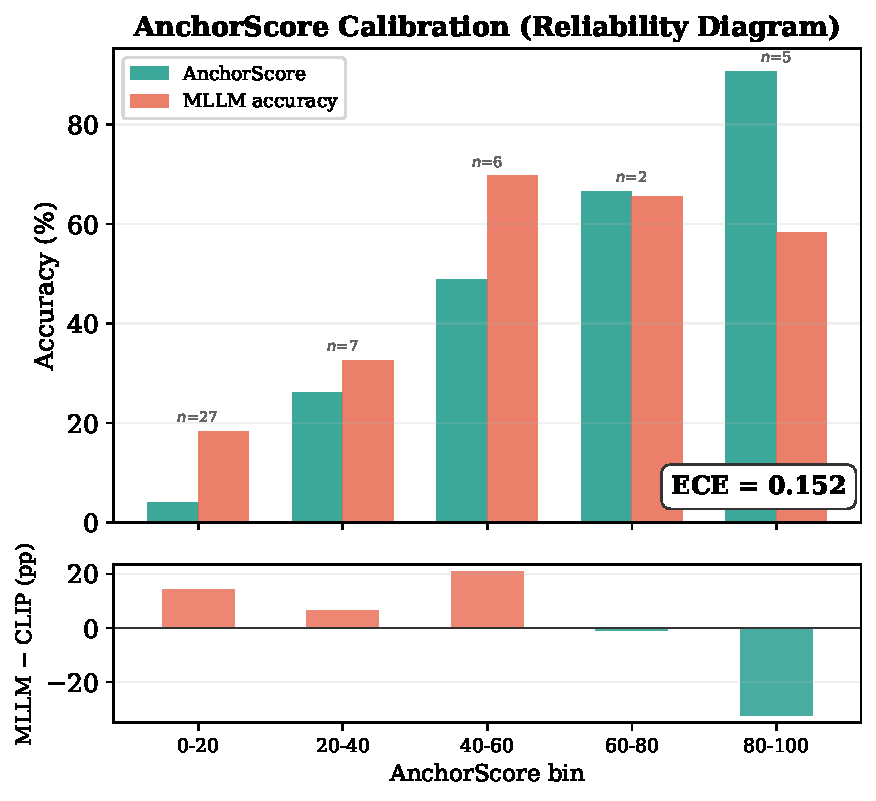
\includegraphics[width=\columnwidth]{figA2_calibration.pdf}
\caption{Calibration plot: AnchorScore vs.\ mean MLLM accuracy across 47 classes (5 bins). Perfect calibration would show equal bar heights per bin; the lower panel quantifies the gap (MLLM $-$ CLIP in pp). The ECE of 0.152 is consistent with AnchorScore supporting ranking, not absolute accuracy estimation.}
\label{fig:calibration}
\end{figure}


%%%%%%%%%%%%%%%%%%%%%%%%%%%%%%%%%%%%%%%%%%
% Author Contributions, etc.
%%%%%%%%%%%%%%%%%%%%%%%%%%%%%%%%%%%%%%%%%%

\section*{Author Contributions}
Conceptualization, L.Z.; methodology, L.Z. and Y.M.; software, L.Z.; validation, L.Z. and Y.M.; formal analysis, L.Z.; investigation, L.Z. and Y.M.; writing---original draft preparation, L.Z.; writing---review and editing, L.Z. and Y.M.; supervision, L.Z. All authors have read and agreed to the published version of the manuscript.

\section*{Data Availability}
The SCB5 datasets used in this study are publicly available on Hugging Face at \url{https://huggingface.co/datasets/wintonYF/SCB-Dataset}. EuroSAT is available at \url{https://github.com/phelber/EuroSAT}. MedMNIST datasets are available at \url{https://medmnist.com}. The experiment code, prompt templates, per-image MLLM predictions, and all result files are available at \url{https://github.com/zhanglizhuo/VisualAnchor}.

\section*{Acknowledgments}
The authors thank the contributors of the SCB dataset, EuroSAT, and MedMNIST for making their data publicly available. During the preparation of this work, the authors used AI-assisted tools for code development and manuscript revision support. After using these tools, the authors reviewed and edited the content as needed and take full responsibility for the content of the publication.

\section*{Conflicts of Interest}
The authors declare no conflicts of interest.


%%%%%%%%%%%%%%%%%%%%%%%%%%%%%%%%%%%%%%%%%%
% References
%%%%%%%%%%%%%%%%%%%%%%%%%%%%%%%%%%%%%%%%%%

\bibliographystyle{IEEEtran}
\bibliography{refs}


%%%%%%%%%%%%%%%%%%%%%%%%%%%%%%%%%%%%%%%%%%
% Biographies
%%%%%%%%%%%%%%%%%%%%%%%%%%%%%%%%%%%%%%%%%%

\begin{IEEEbiographynophoto}{Yan Ma}
received the Ph.D. degree in linguistics from Hunan Normal University. She is currently a lecturer with the School of Foreign Studies, Changsha University of Science and Technology. Her research interests include applied linguistics and educational technology.
\end{IEEEbiographynophoto}

\begin{IEEEbiographynophoto}{Lizhuo Zhang}
received the Ph.D. degree in computer science from Hunan University. He is currently an assistant professor with the School of Information and Intelligence, Hunan Agricultural University. His research interests include multimodal learning, vision-language models, and their applications in educational technology.
\end{IEEEbiographynophoto}

\EOD

\end{document}
